% ============================================================
%  第四章 等离激元（§1–§11 + 参考文献）
%  底本：高等教育出版社《固体理论》第二版；原书印刷页 89–137
%  （PDF 页 = 印刷页 + 20）
%  公式编号：每节自 (4.N.1) 起自动编号，共 255 个编号
%  （其中 (4.9.27)、(4.9.28)、(4.9.30)、(4.11.30) 各分 a/b(/c) 两三式）
%
%  已修正的 OCR 错误：
%  1. §1 章首"集体振荡量子 ħωq"后 OCR 复制的 $\hbar\omega_q$ 已删（对照 p110）；
%     "如图4.1所示"中混入的 q 已删（p111）。
%  2. §2 (4.2.2)(4.2.5)(4.2.6)(4.2.9) 中被拆散的 v(q)、带撇求和号按 p113 修复；
%     (4.2.3) \hat{o}→δ；(4.2.8) \dot{C}→C^+；e²/r 傅里叶展开式原书无编号，
%     OCR 的空 \tag{} 已去掉。
%  3. §3 (4.3.3) "4πe²i/m"、(4.3.5) q·q′/q′² 按 p115 修复；(4.3.7) Σi→Σj。
%  4. §4 (4.4.2) φ→ρ̇；(4.4.8) C^-→C；(4.4.9) 整块按 p117 重排；
%     (4.4.10) \widehat{θ}→δ。
%  5. §5 (4.5.13)(4.5.15) 下标 ι、误入的 \hbar 杂符按 p119–120 修复。
%  6. §6 (4.6.6) 整式按 p122 重排；∈/E/e 等介电函数记号统一为 ε；
%     (4.6.9) (−ε)→(−e)；(4.6.22) \mathfrak{E}→δ；(4.6.24) 句尾杂符已删；
%     (4.6.14) 按原书（p122 底—p123 顶跨页一式）补回首行 ε=Ve/V。
%  7. §6 林哈德 ε1、ε2 显式式（(4.6.25)(4.6.26)）OCR 并作一块且严重乱码，
%     已按 p124 原书页面拆成两式重排。
%  8. §7 (4.7.4) 的编号 OCR 掉到正文，已归还该式（p126）。
%  9. §8 (4.8.7) q0r→qcr；\hat{δ}→δ。
% 10. §9 (4.9.5) 编号 OCR 缺失，按正文引用证实该式即 (4.9.5)（p134）；
%     (4.9.7) 相邻两块 $$ 按原书合并为一式（p134–135）；
%     \hat{δ}/\widehat{⊗}/\mathfrak{d}→δ；(4.9.40) φ/ψ 混用统一为 ψ；
%     (4.9.60) 按原书（p142）补为三行等式（OCR 只存首行）；
%     (4.9.71) 补回 "=" 续行；(4.9.73)(4.9.75)(4.9.77)(4.9.78) 的残缺
%     tag（{73}/(4.9.75)/{.77}/{9.78}）按 p144–145 恢复；
%     (4.9.27)(4.9.28)(4.9.30) 的 a/b 分编号按 p137–138 恢复。
% 11. §10 (4.10.10) 首行分母按 (4.10.4) 应为 2r0（原书印作 2rs，已改并注）。
% 12. §11 (4.11.2)(4.11.4) \hat{⊗}→δ、误入的 \hbar 已删（p149–150）；
%     \tag{1.5}→(4.11.5)；(4.11.30a) 按 p154 重排；T_k→Γ_k；θ_k→g_k；
%     "利费密黄金规则"→"利用费密黄金规则"；p150 脚注①已补录；
%     章首段"[在量子多体理论中称为自能……详见附录C]也是复量"按 p148 恢复。
% 13. 全章：全角句号"．/。"→ ASCII "."；OCR 间隔符 ~ 删除；"5~30 eV"→"5～30 eV"；
%     "F格"→"严格"；"这个积分长在波限"→"这个积分在长波限"（原书倒字）；
%     附录A一D→附录A—D；Kohnanomalies→Kohn anomalies；
%     "求动能部分 对ij^m格基态的平均"→"求动能部分……对严格基态的平均"（p139）。
%  原书排印错误（照页面修正，均已在正文按原样改正）：
%  A. p130 "当 qcr→2 时 Si(qcr)→π/2"→ qcr→∞（物理极限）；
%  B. p130 "库仑势中自然只剩下短波成分 (q<qc)"→ (q>qc)（与上下文物理矛盾）；
%  C. p138 (4.9.30a)(4.9.30b) 的 lim 下标 q→0→ q→∞（上下文为大 q 渐近）；
%  D. p117 (4.4.11) 左端 ρ_{kp}^+→ρ_{kq}^+（按式 (4.4.10) 上下文）；
%  E. p132 (4.8.12) 右端 Z/8π³ 与 4πZe² 重复计 Z，按 (4.8.11) 傅里叶逆
%     改为 1/8π³。
%  遗留问题：
%  · 文献[7] "Solid State Phys, 1995" 系原书如此（史实为 1955），照录未改；
%  · 图4.2 无裁剪图，占位图待重绘代理按原书 p112 绘制；原书图注仅"图 4.2"；
%  · (4.4.11) 原书左端下标 kp/q 印刷难辨，按物理取 kq。
% ============================================================
\chapter{等离激元}

本章讨论在宽能带金属中，当价电子之间存在库仑互作用时的元激发特征.由于库仑互作用的长程性以及价电子易动的巡游性，将导致电子系统既存在集体激发（等离激元），又出现个别激发（准电子），在理论上属于不能严格对角化的多体系统，必须采用近似方法.为了将所研究的体系变为纯粹的电子-电子相互作用系统，在本章中暂时略去晶格周期场和晶格振动（声子）对电子的影响，采用一个简化的金属模型（§2），并介绍一种在高密度条件下可以求解经典及量子运动方程的合理近似——无规相近似（见§3、§4）.在此基础上，我们将采用动态介电函数方法研究相互作用电子系统对含时外扰动的线性响应（§5），并求出无规相近似介电函数（§6），这种新方法的优点是，可以统一求出系统的个别与集体激发（§7），屏蔽效应（§8），并解决金属基态能计算的发散困难.最后，在§11中将证明相互作用电子系统中仍然存在费密面.采用动态介电函数方法的另一优点是，可以通过热力学格林函数直接推广到有限温度情形，因此在学习本章时应同时阅读附录A—D中有关的格林函数介绍.

\section{等离激元和准电子}

先介绍电子-电子互作用系统元激发的物理图像.以金属中的电子为例，价电子在离子的正电抵消背景上运动，系统在宏观尺度上保持着电中性.由于价电子易动，而且电子间有相互作用，因此系统在微观尺度上必然存在着电子密度的起伏.鉴于电子间相互作用是库仑势，具有长程作用的特征，所以哪怕是局域的密度起伏也将在整个系统中产生电子运动的关联，这是一种集体效应.人们常采用系统中电子密度的傅里叶分量 $\rho_{q}$ 作为集体坐标来描述这种关联.与晶格振动问题中的集体坐标相类似，在这里 $\rho_{q}$ 将以波动的形式出现，它是系统中电子密度起伏相对于正电背景的振荡，称为等离子区集体振荡.波矢为 $\boldsymbol{q}$ 频率为 $\omega_{q}$ 的等离子区集体振荡量子 $\hbar\omega_{q}$，在固体物理中，叫做等离激元（plasmons）.等离激元的频率在长波长时容易求出，此时可设每个电子相对于正离子背景的移动均为 $x$，电子移动后所产生的电场
\begin{equation*}
  \mathcal{E}=4\pi Nex
\end{equation*}
$N$ 是单位体积中的价电子数，于是作用于每个电子上的恢复力为 $-e\mathcal{E}$，电子运动满足方程
\begin{equation*}
  m\ddot{x}=-4\pi Ne^{2}x
\end{equation*}
显然，每一个电子均以相同的频率
\begin{equation}
  \omega_{\mathrm{p}}^{2}=\frac{4\pi Ne^{2}}{m}
\end{equation}
振荡，$\hbar\omega_{\mathrm{p}}$ 一般为 5～30 eV.在本章中我们将利用二次量子化工具较严格的确定每个波矢 $\boldsymbol{q}$ 对应的等离激元能量 $\hbar\omega_{q}$，求出其色散关系.式(4.1.1)仅仅是 $q=0$ 时的频率.

除集体激发以外，金属中还存在电子的个别激发.讨论金属中电子的个别行为时，必须考虑费密面的存在，这时从 $\boldsymbol{k}$ 空间分析问题图像更为清楚.系统的“真空”（即基态）可近似描述为在费密球 $k_{\mathrm{F}}$ 内的所有状态均被电子占据，而球外则全空着.相对于这个“真空”的个别激发是从费密球内 $\boldsymbol{k}$ 态上拿出一个电子放到球外 $\boldsymbol{k}+\boldsymbol{q}$ 空状态上去，于是在金属的“真空”上产生了一个 $\boldsymbol{k}+\boldsymbol{q}$ 电子和一个 $\boldsymbol{k}$ 空穴，这种电子和空穴对的个别激发能量记作
\begin{equation}
  \hbar\omega_{kq}=\frac{\hbar^{2}(\boldsymbol{k}+\boldsymbol{q})^{2}}{2m}
  -\frac{\hbar^{2}k^{2}}{2m}
  =\frac{\hbar^{2}}{2m}\left(q^{2}+2\boldsymbol{k}\cdot\boldsymbol{q}\right)
\end{equation}
对于确定的 $\boldsymbol{q}$，存在着一个受泡利原理限制的许可区域，如图4.1所示.

\begin{center}
\begin{minipage}{8.5cm}
\centering
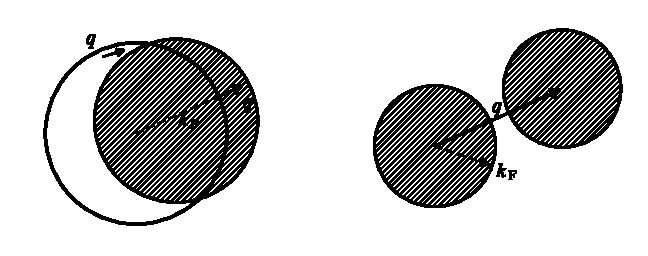
\includegraphics[width=8.5cm]{fig4-1.pdf}\\[0.3em]
{\small (a) $q<2k_{\mathrm{F}}$\qquad\qquad (b) $q>2k_{\mathrm{F}}$}\\[0.2em]
{\small 图 4.1}
\end{minipage}
\end{center}

（i）$q<2k_{\mathrm{F}}$：此时并非球内每个电子都可激发到球外，只有图4.1(a)中两个弯月形才是许可的区域，其中内层的阴影区是空穴激发区，外层的阴影区代表电子激发区.由图还可以定出激发能 $\hbar\omega_{kq}$ 的界限为
\begin{equation}
  \hbar\omega_{kq}^{\max}=\frac{\hbar^{2}}{2m}\left(q^{2}+2k_{\mathrm{F}}q\right);\quad
  \hbar\omega_{kq}^{\min}=0
\end{equation}
（ii）$q>2k_{\mathrm{F}}$：费密球内全为空穴激发区，另一个原点在 $\boldsymbol{q}$ 的球内［见图4.1(b)］是电子激发区，对应 $\hbar\omega_{kq}$ 的界限为
\begin{equation}
  \hbar\omega_{kq}^{\max}=\frac{\hbar^{2}}{2m}\left(q^{2}+2k_{\mathrm{F}}q\right);\quad
  \hbar\omega_{kq}^{\min}=\frac{\hbar^{2}}{2m}\left(q^{2}-2k_{\mathrm{F}}q\right)
\end{equation}
图4.2中注明的对激发区，是按照公式(4.1.3)和(4.1.4)作出的，在同一图中也绘出了等离激元的色散曲线 $\omega_{q}$.在§5中将证明等离激元的长波色散关系为
\begin{equation}
  \omega_{q}=\omega_{\mathrm{p}}+\frac{3v_{\mathrm{F}}^{2}q^{2}}{10\omega_{\mathrm{p}}}
\end{equation}
其中 $v_{\mathrm{F}}$ 为费密速度，$v_{\mathrm{F}}=\hbar k_{\mathrm{F}}/m$.

\begin{center}
\begin{minipage}{5.5cm}
\centering
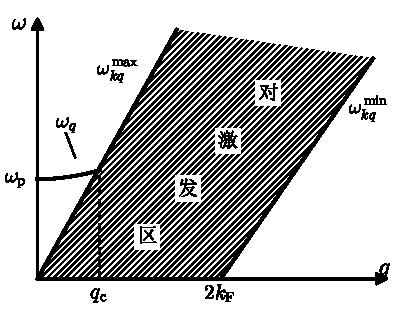
\includegraphics[width=5.5cm]{fig4-2.pdf}\\{\small 图 4.2}
\end{minipage}
\end{center}

由图4.2可以看出，存在着集体振荡与电子-空穴时个别激发区的交点 $q_{c}$.当 $q<q_{c}$ 时，等离激元能量 $\hbar\omega_{q}$ 大于电子-空穴对个别激发的最大能量 $\hbar\omega_{kq}^{\max}$，集体振荡既不可能被个别对所激发，也不可能衰减为个别的电子-空穴对.但是，当 $q>q_{c}$ 时由于 $\hbar\omega_{kq}^{\max}>\hbar\omega_{q}$，将出现振荡的衰减.在§5中我们将分析电子系统的介电函数，并证明 $q>q_{c}$ 时等离子区集体振荡是不稳定的.因此，仅仅在长波范围 $0<q<q_{c}$ 之内，才有集体激发（等离激元）存在，而当 $q>q_{c}$ 时，只有个别对激发，$q_{c}$ 可认为是划分金属电子系统个别激发与集体激发的特性参量.在相互作用电子系统中，长波范围（小 $q$）内主要是集体振荡，短波（大 $q$）时为普通的电子-空穴对激发.

电子间相互作用对于金属中个别电子的性能也有影响，其中特别重要的是屏蔽效应，库仑作用使得每个电子周围形成了正电荷的屏蔽壳层，它跟随着激发它的电子一起运动，从而改变电子间的相互作用势和电子的有效质量.人们把（电子$+$屏蔽电荷）的整体称为准电子（quasi-electrons）.准电子间互作用不再是库仑势，而是汤川型屏蔽库仑势 $\dfrac{e^{2}}{r}\mathrm{e}^{-\lambda r}$，$\lambda$ 与 $q_{c}$ 同量级（见§8）.因此，准电子间的有效互作用近似为 $\dfrac{e^{2}}{r}\mathrm{e}^{-q_{c}r}$，它与 $\displaystyle\sum_{q>q_{c}}\frac{4\pi e^{2}}{q^{2}}\mathrm{e}^{\mathrm{i}\boldsymbol{q}\cdot\boldsymbol{r}}$ 大致相同，说明互作用来自库仑势 $\dfrac{e^{2}}{r}$ 展开的短波部分.显然，库仑势展开的长波部分被扣除了，这是因为库仑作用的长程部分已用于电子系统的集体振荡.

\section{互作用电子系统的哈密顿量}

当讨论金属中电子的元激发特征时，能带效应并不重要.可以把排成晶格的正离子近似当作是均匀抹平了的连续正电荷分布，像凝胶（jellium）一样.公有化电子则在此正电荷背景上运动，整个系统保持电中性.这种简化的金属电子模型称为凝胶模型.

电子体系的哈密顿量为
\begin{equation}
  H=-\sum_{i=1}^{N}\frac{\hbar^{2}\nabla_{i}^{2}}{2m}
  +\frac{1}{2}\mathop{{\sum}'}\limits_{i,j}\frac{e^{2}}{|\boldsymbol{r}_{i}-\boldsymbol{r}_{j}|}
  +H_{+}
\end{equation}
其中 $H_{+}$ 是均匀分布正电荷背景的贡献项，包括正电背景的自作用能以及它与电子的互作用能.为简单起见，设公有化电子数为 $N$，并取单位体积样品 $V=1$，将 $e^{2}/r$ 作傅里叶展开
\begin{equation*}
  \frac{e^{2}}{r}=\sum_{\boldsymbol{q}}v(\boldsymbol{q})\mathrm{e}^{\mathrm{i}\boldsymbol{q}\cdot\boldsymbol{r}},
  \quad v(\boldsymbol{q})=\frac{4\pi e^{2}}{q^{2}}
\end{equation*}
则
\begin{equation}
  H=-\sum_{i=1}^{N}\frac{\hbar^{2}\nabla_{i}^{2}}{2m}
  +\frac{1}{2}\sum_{\boldsymbol{q}}\mathop{{\sum}'}\limits_{i,j}
  v(\boldsymbol{q})\mathrm{e}^{\mathrm{i}\boldsymbol{q}\cdot(\boldsymbol{r}_{i}-\boldsymbol{r}_{j})}
  +H_{+}
\end{equation}
根据§1中讨论，用电子密度的傅里叶分量表示 $H$，由于电子的密度
\begin{equation}
  \rho(\boldsymbol{r})=\sum_{j}\delta(\boldsymbol{r}-\boldsymbol{r}_{j})
  =\sum_{\boldsymbol{q}}\sum_{j}\mathrm{e}^{\mathrm{i}\boldsymbol{q}\cdot(\boldsymbol{r}-\boldsymbol{r}_{j})}
  \equiv\sum_{\boldsymbol{q}}\rho_{q}\mathrm{e}^{\mathrm{i}\boldsymbol{q}\cdot\boldsymbol{r}}
\end{equation}
因此密度 $\rho(\boldsymbol{r})$ 的傅里叶分量为
\begin{equation}
  \rho_{q}=\sum_{j}\mathrm{e}^{-\mathrm{i}\boldsymbol{q}\cdot\boldsymbol{r}_{j}},\quad
  \rho_{q}^{+}=\sum_{j}\mathrm{e}^{\mathrm{i}\boldsymbol{q}\cdot\boldsymbol{r}_{j}}=\rho_{-q}
\end{equation}
代入式(4.2.2)得到
\begin{equation}
  H=-\sum_{i=1}^{N}\frac{\hbar^{2}\nabla_{i}^{2}}{2m}
  +\frac{1}{2}\sum_{q}v(q)\left(\rho_{q}^{+}\rho_{q}-N\right)+H_{+}
\end{equation}
其中 $-\dfrac{1}{2}v(q)N$ 为扣除的 $i=j$ 项，第二个求和项中的 $q=0$ 部分代表均匀分布的电子自作用能，在凝胶模型中恰好与 $H_{+}$ 相抵消.因此，在哈密顿量中可略去 $H_{+}$，只取 $q\neq 0$ 项，这时 $\rho_{q}$ 代表密度起伏.
\begin{equation}
  H=-\sum_{i=1}^{N}\frac{\hbar^{2}\nabla_{i}^{2}}{2m}
  +\frac{1}{2}\mathop{{\sum}'}\limits_{q}v(q)\left(\rho_{q}^{+}\rho_{q}-N\right)
\end{equation}
这就是凝胶模型中电子系统的哈密顿量.

在二次量子化表象中，$\rho_{q}$ 与 $\rho_{q}^{+}$ 对应于密度起伏算符，有关系式
\begin{equation}
\begin{aligned}
  \rho(\boldsymbol{r},t)
  &=\int\varPsi^{+}(\boldsymbol{r}',t)\delta(\boldsymbol{r}-\boldsymbol{r}')
  \varPsi(\boldsymbol{r}',t)\,\mathrm{d}\boldsymbol{r}'\\
  &=\varPsi^{+}(\boldsymbol{r},t)\varPsi(\boldsymbol{r},t)\\
  &=\sum_{k,k'}C_{k}^{+}C_{k'}\mathrm{e}^{-\mathrm{i}(\boldsymbol{k}-\boldsymbol{k}')\cdot\boldsymbol{r}}\\
  &=\sum_{k,q}C_{k}^{+}C_{k+q}\mathrm{e}^{\mathrm{i}\boldsymbol{q}\cdot\boldsymbol{r}}
  \qquad\left(\boldsymbol{q}\equiv\boldsymbol{k}'-\boldsymbol{k}\right)
\end{aligned}
\end{equation}
由此求得 $\rho_{q}$、$\rho_{q}^{+}$ 与产生及消灭算符 $C_{k}^{+}$、$C_{k'}$ 的关系为：
\begin{equation}
  \left.\begin{aligned}
  \rho_{q}&=\sum_{k}C_{k}^{+}C_{k+q}=\sum_{k}C_{k-q}^{+}C_{k}\\
  \rho_{q}^{+}&=\sum_{k}C_{k+q}^{+}C_{k}=\rho_{-q}
  \end{aligned}\right\}
\end{equation}
则哈密顿量
\begin{equation}
  H=\sum_{k}E_{k}C_{k}^{+}C_{k}
  +\frac{1}{2}\mathop{{\sum}'}\limits_{q}v(q)\left(\rho_{q}^{+}\rho_{q}-N\right)
\end{equation}
其中 $E_{k}=\hbar^{2}k^{2}/2m$，$C_{k}$ 与 $C_{k}^{+}$ 满足费密子反对易式
\begin{equation}
  \left.\begin{aligned}
  [\,C_{k},C_{k'}^{+}\,]_{+}&=C_{k}C_{k'}^{+}+C_{k'}^{+}C_{k}=\delta_{kk'}\\
  [\,C_{k},C_{k'}\,]_{+}&=[\,C_{k}^{+},C_{k'}^{+}\,]_{+}=0
  \end{aligned}\right\}
\end{equation}
为简单起见，在以上表示式中没有明确写出电子的自旋标记 $\sigma$，实际上
\begin{equation}
  \rho_{q}=\sum_{k,\sigma}C_{k-q,\sigma}^{+}C_{k\sigma},\quad
  \rho_{q}^{+}=\sum_{k,\sigma}C_{k+q,\sigma}^{+}C_{k,\sigma}
\end{equation}
而总哈密顿量为
\begin{equation}
\begin{aligned}
  H&=\sum_{k,\sigma}E_{k}C_{k\sigma}^{+}C_{k\sigma}
  +\frac{1}{2}\mathop{{\sum}'}\limits_{q}v(q)\left(\rho_{q}^{+}\rho_{q}-N\right)\\
  &=\sum_{k,\sigma}E_{k}C_{k\sigma}^{+}C_{k\sigma}
  +\frac{1}{2}\mathop{{\sum}'}\limits_{q}\sum_{k,k'}\sum_{\sigma,\sigma'}
  v(q)C_{k+q,\sigma}^{+}C_{k'-q,\sigma'}^{+}C_{k'\sigma'}C_{k\sigma}
\end{aligned}
\end{equation}
与通常的标准形式一样.

\section{电子集体振荡的经典理论}

讨论经典情况的目的，是为了介绍求解电子等离子集体振荡的合理近似方法.

式(4.2.3)对时间求导，得
\begin{equation}
  \dot{\rho}_{q}=-\mathrm{i}\sum_{j}\boldsymbol{q}\cdot\boldsymbol{v}_{j}\,
  \mathrm{e}^{-\mathrm{i}\boldsymbol{q}\cdot\boldsymbol{r}_{j}}
\end{equation}
这里 $\boldsymbol{v}_{j}=\dot{\boldsymbol{r}}_{j}$ 是第 $j$ 个电子的速度，再求导，得方程
\begin{equation}
  \ddot{\rho}_{q}=-\sum_{j}\left\{\left(\boldsymbol{q}\cdot\boldsymbol{v}_{j}\right)^{2}
  +\mathrm{i}\boldsymbol{q}\cdot\dot{\boldsymbol{v}}_{j}\right\}
  \mathrm{e}^{-\mathrm{i}\boldsymbol{q}\cdot\boldsymbol{r}_{j}}
\end{equation}
$\dot{\boldsymbol{v}}_{j}$ 由经典力学方程决定
\begin{equation}
  \dot{\boldsymbol{v}}_{j}=-\frac{1}{m}\nabla_{j}
  \left\{\frac{1}{2}\mathop{{\sum}'}\limits_{q'}v(q')
  \left(\rho_{q'}^{+}\rho_{q'}-N\right)\right\}
  =-\frac{4\pi e^{2}\mathrm{i}}{m}\mathop{{\sum}'}\limits_{q'}
  \frac{\boldsymbol{q}'}{q'^{2}}\rho_{q'}\mathrm{e}^{\mathrm{i}\boldsymbol{q}'\cdot\boldsymbol{r}_{j}}
\end{equation}
其中 $\mathop{{\sum}'}\limits_{q'}$ 表示限制 $q'\neq 0$，是由于考虑了电子体系中均匀正电背景的影响.将 $\dot{\boldsymbol{v}}_{i}$ 代入 $\ddot{\rho}_{q}$ 方程，求得电子密度的傅里叶分量 $\rho_{q}$ 满足下列非线性的运动方程：
\begin{equation}
  \ddot{\rho}_{q}=-\sum_{j}\left(\boldsymbol{q}\cdot\boldsymbol{v}_{j}\right)^{2}
  \mathrm{e}^{-\mathrm{i}\boldsymbol{q}\cdot\boldsymbol{r}_{j}}
  -\left(\frac{4\pi e^{2}}{m}\right)\mathop{{\sum}'}\limits_{q'}
  \frac{\boldsymbol{q}\cdot\boldsymbol{q}'}{q'^{2}}\rho_{q'}\rho_{q-q'}
\end{equation}
上式中右边第二项又可分成 $\boldsymbol{q}'=\boldsymbol{q}$ 和 $\boldsymbol{q}'\neq\boldsymbol{q}$ 两部分：
\begin{equation}
  -\left(\frac{4\pi e^{2}}{m}\right)
  \left\{N\rho_{q}+\mathop{{\sum}'}\limits_{q'(q'\neq q)}
  \frac{\boldsymbol{q}\cdot\boldsymbol{q}'}{q'^{2}}\rho_{q'}\rho_{q-q'}\right\}
\end{equation}
假如略去 $\boldsymbol{q}'\neq\boldsymbol{q}$ 项，只保留 $\boldsymbol{q}'=\boldsymbol{q}$ 项，则可将式(4.3.4)线性化为
\begin{equation}
  \ddot{\rho}_{q}=-\sum_{j}\left\{\frac{4\pi Ne^{2}}{m}
  +\left(\boldsymbol{q}\cdot\boldsymbol{v}_{j}\right)^{2}\right\}
  \mathrm{e}^{-\mathrm{i}\boldsymbol{q}\cdot\boldsymbol{r}_{j}}
\end{equation}
或
\begin{equation}
  \ddot{\rho}_{q}+\omega_{\mathrm{p}}^{2}\rho_{q}
  =-\sum_{j}\left(\boldsymbol{q}\cdot\boldsymbol{v}_{j}\right)^{2}
  \mathrm{e}^{-\mathrm{i}\boldsymbol{q}\cdot\boldsymbol{r}_{j}}
\end{equation}
当 $\boldsymbol{q}\to 0$ 时，可略去 $\left(\boldsymbol{q}\cdot\boldsymbol{v}_{j}\right)^{2}$ 项，求得 $\rho_{q}$ 的简谐振动方程
\begin{equation}
  \ddot{\rho}_{q}+\omega_{\mathrm{p}}^{2}\rho_{q}=0\quad(q\to 0)
\end{equation}
其中 $\omega_{\mathrm{p}}^{2}=\dfrac{4\pi Ne^{2}}{m}$ 是在长波限的等离子振荡频率，色散关系也可由方程(4.3.7)求出.

显然，在以上求解过程中主要的近似为，在式(4.3.5)中略去两个不同密度起伏模 $\rho_{q'}$ 与 $\rho_{q-q'}$ 之间的耦合项，其理由如下：由于 $\rho_{q}=\displaystyle\sum_{j}\mathrm{e}^{-\mathrm{i}\boldsymbol{q}\cdot\boldsymbol{r}_{j}}$ 是指数项之和，而这些指数的相位因子又由 $\boldsymbol{r}_{j}$ 决定，对于高密度电子系统，电子的位置在空间的分布是杂乱无规的，这时 $\rho_{q}\ (q\neq 0)$ 代表相位无规变化的指数项之和，对于平移不变的系统其平均值为零，所以两个密度起伏的乘积项对于运动方程(4.3.4)仅仅是微小的修正，作为一级近似可略去，这样的近似称为无规相近似（RPA）.这里无规相的含义正在于 $\rho_{q}$ 是无规相位的指数相加，而 $\rho_{0}=N$ 是各项的相干叠加，两者在高密度条件下相差很大.所以，式(4.3.5)中 $\rho_{q'}\rho_{q-q'}$ 相对于 $N\rho_{q}$ 是小量，略去它是合理的.

\section{量子运动方程的无规相近似}

我们将从算符的运动方程出发，求解互作用电子体系的近似本征值.定义电子-空穴对的激发算符
\begin{equation}
  \rho_{kq}^{+}\equiv C_{k+q}^{+}C_{k}
\end{equation}
$\rho_{kq}^{+}$ 作用于系统的“真空”，相当在费密球内 $\boldsymbol{k}$ 态上产生一个空穴，在球外 $\boldsymbol{k}+\boldsymbol{q}$ 态上产生一个电子，代表金属中的个别激发.在互作用电子系统中这些个别激发是彼此耦合在一起的，算符 $\rho_{kq}$ 及 $\rho_{kq}^{+}$ 的海森伯运动方程为
\begin{equation}
  -\mathrm{i}\hbar\dot{\rho}_{kq}=[H,\rho_{kq}];\quad
  -\mathrm{i}\hbar\dot{\rho}_{kq}^{+}=[H,\rho_{kq}^{+}]
\end{equation}
根据式(4.2.8)密度起伏 $\rho_{q}$，$\rho_{q}^{+}$ 是总动量为 $\hbar\boldsymbol{q}$ 的所有电子-空穴对运动的简单叠加
\begin{equation}
  \rho_{q}^{+}=\sum_{k}\rho_{kq}^{+}
\end{equation}
我们只要能解出电子-空穴对的运动方程(4.4.2)，则电子体系的元激发谱就求得了.

$\rho_{kq}^{+}$ 的本征方程为
\begin{equation}
  \left[H,\rho_{kq}^{+}\right]=\hbar\omega\rho_{kq}^{+}
\end{equation}
将上式代入方程(4.4.2)，得到 $-\mathrm{i}\hbar\dot{\rho}_{kq}^{+}=\hbar\omega\rho_{kq}^{+}$，说明 $\hbar\omega$ 代表能量本征值，而式(4.4.4)即类似于式(3.6.7)的运动方程的对角化条件.

式(4.4.2)或(4.4.4)是电子-空穴对激发的耦合方程.假如不存在相互作用，即 $\boldsymbol{v}(\boldsymbol{q})=0$，则 $H=\displaystyle\sum_{k}E_{k}C_{k}^{+}C_{k}\equiv H_{0}$ 代表独立电子系统，这时容易求得
\begin{equation}
  \left[H_{0},\rho_{kq}^{+}\right]
  =\left\{\frac{\hbar^{2}}{2m}(\boldsymbol{k}+\boldsymbol{q})^{2}
  -\frac{\hbar^{2}}{2m}k^{2}\right\}\rho_{kq}^{+}
  =\hbar\omega_{kq}\rho_{kq}^{+}
\end{equation}
这里 $\hbar\omega_{kq}$ 正如式(4.1.2)所定义，是不计相互作用时电子-空穴对的激发能量，代表电子-空穴的自由传播.

对于互作用电子体系 $\boldsymbol{v}(\boldsymbol{q})\neq 0$，上述对易式较复杂：
\begin{equation}
  \left[H,\rho_{kq}^{+}\right]=\hbar\omega_{kq}\rho_{kq}^{+}
  +\frac{1}{2}\mathop{{\sum}'}\limits_{q'}v(q')
  \big\{\left[\,\rho_{q'}^{+},\rho_{kq}^{+}\,\right]\rho_{q'}
  +\rho_{q'}^{+}\left[\,\rho_{q'},\rho_{kq}^{+}\,\right]\big\}
\end{equation}
由于 $\boldsymbol{v}(\boldsymbol{q})=\boldsymbol{v}(-\boldsymbol{q})$，$\rho_{q}^{+}=\rho_{-q}$，上式可改写为
\begin{equation}
  \left[H,\rho_{kq}^{+}\right]=\hbar\omega_{kq}\rho_{kq}^{+}
  +\frac{1}{2}\mathop{{\sum}'}\limits_{q'}v(q')
  \big\{\left[\,\rho_{q'},\rho_{kq}^{+}\,\right]\rho_{q'}^{+}
  +\rho_{q'}^{+}\left[\,\rho_{q'},\rho_{kq}^{+}\,\right]\big\}
\end{equation}
利用 $\left[A,BC\right]=\left[A,B\right]_{+}C-B\left[A,C\right]_{+}$，算出对易式
\begin{equation}
\begin{aligned}
  \left[\rho_{q'},\rho_{kq}^{+}\right]
  &=\Big[\sum_{k'}C_{k'-q'}^{+}C_{k'},C_{k+q}^{+}C_{k}\Big]\\
  &=C_{k+q-q'}^{+}C_{k}-C_{k+q}^{+}C_{k+q'}
\end{aligned}
\end{equation}
代入式(4.4.7)，并分出 $\boldsymbol{q}'=\boldsymbol{q}$ 与 $\boldsymbol{q}'\neq\boldsymbol{q}$ 项，整理后写成
\begin{equation}
\begin{aligned}
  \left[H,\rho_{kq}^{+}\right]={}&\hbar\omega_{kq}\rho_{kq}^{+}
  +\frac{1}{2}v(q)\big\{\big(C_{k}^{+}C_{k}-C_{k+q}^{+}C_{k+q}\big)\sum_{k'}\rho_{k'q}^{+}\\
  &+\sum_{k'}\rho_{k'q}^{+}\big(C_{k}^{+}C_{k}-C_{k+q}^{+}C_{k+q}\big)\big\}\\
  &+\frac{1}{2}\mathop{{\sum}'}\limits_{q'(q'\neq q)}v(q')
  \big\{\big(C_{k+q-q'}^{+}C_{k}-C_{k+q}^{+}C_{k+q'}\big)\rho_{q'}^{+}\\
  &\quad+\rho_{q'}^{+}\big(C_{k+q-q'}^{+}C_{k}-C_{k+q}^{+}C_{k+q'}\big)\big\}
\end{aligned}
\end{equation}
式(4.4.9)中右边第一项代表自由运动，第二项是具有相同 $\boldsymbol{q}$ 的所有电子-空穴对间的耦合，最后的求和项为不同 $\boldsymbol{q}$ 的电子-空穴对之间的相互作用，它表明一个总动量 $\hbar\boldsymbol{q}$ 的对将激发另一组 $\hbar\boldsymbol{q}'\,(\boldsymbol{q}'\neq\boldsymbol{q})$ 的电子-空穴对.若将第二项称为同“类”对间耦合，则第三项相当于异“类”$(\boldsymbol{q}'\neq\boldsymbol{q})$ 对之间的彼此激发，它们都属于 $\rho_{kq}^{+}$ 本征方程中的非线性部分，为了使算符方程(4.4.4)易于求解，我们将用下列线性化手续：

将式(4.4.8)中算符近似用其对“真空”态的平均值代替
\begin{equation}
\begin{aligned}
  \left[\rho_{q'},\rho_{kq}^{+}\right]
  &=\big(\langle C_{k+q-q'}^{+}C_{k}\rangle_{0}
  -\langle C_{k+q}^{+}C_{k+q'}\rangle_{0}\big)\\
  &=\big(\langle C_{k}^{+}C_{k}\rangle_{0}
  -\langle C_{k+q}^{+}C_{k+q}\rangle_{0}\big)\delta_{qq'}\\
  &=2\left(n_{k}-n_{k+q}\right)\delta_{qq'}
\end{aligned}
\end{equation}
这里由于平移对称性要求动量守恒.因此，只有同类对 $\boldsymbol{q}'=\boldsymbol{q}$ 项有贡献，而异“类”对间的激发自然被消去了，说明后者仅代表更高阶的互作用.这样式(4.4.9)线性化为
\begin{equation}
  \left[H,\rho_{kq}^{+}\right]=\hbar\omega_{kq}\rho_{kq}^{+}
  +2v(q)\left(n_{k}-n_{k+q}\right)\rho_{q}^{+}
\end{equation}
代入式(4.4.4)得到线性化的本征方程
\begin{equation}
  \hbar\left(\omega-\omega_{kq}\right)\rho_{kq}^{+}
  =2v(q)\left(n_{k}-n_{k+q}\right)\rho_{q}^{+}
\end{equation}
上式对 $k$ 求和，再利用式(4.4.3)消去 $\rho_{q}^{+}$，得到频率方程
\begin{equation}
  v(q)\sum_{k}\frac{2\left(n_{k}-n_{k+q}\right)}
  {\hbar\left(\omega-\omega_{kq}\right)}=1
\end{equation}
式中 $2n_{k}$ 是对真空态的平均
\begin{equation}
  \langle C_{k}^{+}C_{k}\rangle_{0}\equiv 2n_{k}=2\theta\left(k_{\mathrm{F}}-k\right)
\end{equation}
其中 $\theta(x)$ 为阶跃函数，真空态指的是自由电子的费密球分布状态，因子2来源于 $k$ 态上自旋简并，因为 $\langle C_{k}^{+}C_{k}\rangle_{0}$ 实际上代表 $\sum\limits_{\sigma}\langle C_{k\sigma}^{+}C_{k\sigma}\rangle_{0}$.式(4.4.13)可作图求解，这里暂不讨论，留待§5中引入电子体系的介电函数以后再作交待.

我们要强调指出：上述线性化手续使运动方程中的 $\boldsymbol{q}'\neq\boldsymbol{q}$ 项自动消除，它与经典情况下的无规相近似实质上是相同的，可称为量子无规相近似.无规相近似在格林函数理论中等效于环形图求和近似，读者可参考《量子统计的格林函数理论》，在那里对无规相近似作了更详细的分析\textsuperscript{[1]}.

为了使问题处理得更为全面起见，我们暂不讨论本征方程(4.4.11)的解，而是先研究系统在外场作用下的变化.这样做既能求得系统的元激发谱，又可得知系统对外扰动的响应.为此，需要先介绍线性响应理论.

\section{\texorpdfstring{线性响应理论\textsuperscript{[2]}}{线性响应理论[2]}}

为了知道给定物理系统的特性，必须以某种方式扰动系统（如加外场或用粒子辐照等方式），然后观察系统的物理量因外加扰动所引起的改变——响应.通过扰动与响应的关系可得知系统的元激发的信息.

设所考虑多粒子系统的哈密顿量为 $H$，它的能量本征值与本征函数分别为 $E_{n}$ 与 $\phi_{n}$，当外场作用于系统时的附加哈密顿量设为 $H_{\mathrm{e}}(t)$.为使响应绝热追随扰动，往往考虑外场缓慢加上，即要求（i）$H_{\mathrm{e}}(t\to-\infty)=0$；（ii）在 $H_{\mathrm{e}}(t)$ 中引入比例因子 $\mathrm{e}^{\eta t}$、$\eta$ 为小正量，计算完成后取 $\eta\to+0$ 极限.

加外场后系统的薛定谔方程为
\begin{equation}
  \mathrm{i}\hbar\frac{\partial\psi}{\partial t}
  =H\psi+H_{\mathrm{e}}(t)\psi
\end{equation}
作变换
\begin{equation}
  \psi(t)=\exp\left(-\frac{\mathrm{i}}{\hbar}Ht\right)\varphi(t)
\end{equation}
可消去 $H$，得更简方程
\begin{equation}
  \frac{\partial\varphi}{\partial t}
  =\frac{1}{\mathrm{i}\hbar}H_{\mathrm{e}}'(t)\varphi
\end{equation}
其中
\begin{equation}
  H_{\mathrm{e}}'(t)=\exp\left(\frac{\mathrm{i}}{\hbar}Ht\right)H_{\mathrm{e}}(t)
  \exp\left(-\frac{\mathrm{i}}{\hbar}Ht\right)
\end{equation}
先考虑纯态情况，设 $t\to-\infty$ 时 $\varphi(t)=\phi_{m}$，则 $\varphi(t)$ 的积分表示为
\begin{equation}
  \varphi(t)=\phi_{m}+\frac{1}{\mathrm{i}\hbar}
  \int_{-\infty}^{t}H_{\mathrm{e}}'(t')\varphi(t')\,\mathrm{d}t'
\end{equation}
若通过物理量 $A$ 观察系统对外场的响应，则算符 $A$ 在 $t$ 时刻的量子力学期待值
\begin{equation}
\begin{aligned}
  \overline{A}&=\int\psi^{*}A\psi\,\mathrm{d}\tau\\
  &=\int\varphi^{*}\exp\Big(\frac{\mathrm{i}}{\hbar}Ht\Big)A
  \exp\Big(-\frac{\mathrm{i}}{\hbar}Ht\Big)\varphi\,\mathrm{d}\tau\\
  &=\int\varphi^{*}A(t)\varphi\,\mathrm{d}\tau
\end{aligned}
\end{equation}
其中
\begin{equation}
  A(t)\equiv\exp\left(\frac{\mathrm{i}}{\hbar}Ht\right)A
  \exp\left(-\frac{\mathrm{i}}{\hbar}Ht\right)
\end{equation}
是算符 $A$ 的海森伯绘景.

必须先解得 $\varphi$，才能计算 $\overline{A}$、$\varphi$ 所满足的积分方程可迭代求解，$\varphi(t)$ 准至 $H_{\mathrm{e}}'(t)$ 线性项的解为
\begin{equation}
  \varphi(t)=\phi_{m}+\frac{1}{\mathrm{i}\hbar}
  \int_{-\infty}^{t}H_{\mathrm{e}}'(t')\phi_{m}\,\mathrm{d}t'
\end{equation}
将上式代入式(4.5.6)求得
\begin{equation}
  \overline{A}=\int\phi_{m}^{*}A(t)\phi_{m}\,\mathrm{d}\tau
  +\frac{1}{\mathrm{i}\hbar}\int_{-\infty}^{t}\mathrm{d}t'
  \int\phi_{m}^{*}\left[A(t),H_{\mathrm{e}}'(t')\right]\phi_{m}\,\mathrm{d}\tau
\end{equation}
由于
\begin{equation*}
  \exp\left(-\frac{\mathrm{i}}{\hbar}Ht\right)\phi_{m}
  =\exp\left(-\frac{\mathrm{i}}{\hbar}E_{m}t\right)\phi_{m}
\end{equation*}
式(4.5.9)右边第一项可化简
\begin{equation}
\begin{aligned}
  \int\phi_{m}^{*}A(t)\phi_{m}\,\mathrm{d}\tau
  &=\int\big(\mathrm{e}^{-\frac{\mathrm{i}}{\hbar}Ht}\phi_{m}\big)^{*}
  A\big(\mathrm{e}^{-\frac{\mathrm{i}}{\hbar}Ht}\phi_{m}\big)\mathrm{d}\tau\\
  &=\int\phi_{m}^{*}A\phi_{m}\,\mathrm{d}\tau=\langle m|A|m\rangle
\end{aligned}
\end{equation}
$\langle m|A|m\rangle$ 是算符 $A$ 对于未受外场扰动状态的平均，这里采用了狄拉克记号.式(4.5.9)相应的改写为
\begin{equation}
  \overline{A}\equiv\langle m|A|m\rangle
  +\frac{1}{\mathrm{i}\hbar}\int_{-\infty}^{t}\mathrm{d}t'\,
  \langle m|\left[A(t),H_{\mathrm{e}}'(t')\right]|m\rangle
\end{equation}
真正观测到的响应，自然不会是上述纯态的平均，而应当是统计平均.因此，进一步设 $t\to-\infty$ 时系统处于热平衡，它在 $\phi_{m}$ 态的概率（probability）为 $w_{m}$，在外场作用下 $t$ 时刻物理量的统计平均值
\begin{equation}
  \langle A\rangle_{t}=\sum_{m}w_{m}\overline{A}
\end{equation}
由式(4.5.11)求得外场所导致系统力学量 $A$ 的统计平均值的改变为
\begin{equation}
  \Delta A\equiv\langle A\rangle_{t}-\langle A\rangle_{t=-\infty}
  =-\frac{\mathrm{i}}{\hbar}\int_{-\infty}^{t}\mathrm{d}t'\,
  \langle\left[A(t),H_{\mathrm{e}}'(t')\right]\rangle
\end{equation}
$\Delta A$ 就是响应.$\langle A\rangle_{t=-\infty}$ 是无外场时 $A$ 的统计平均值.

若外场以频率 $\omega$ 振荡，则附加哈密顿量可设为
\begin{equation}
  H_{\mathrm{e}}(t)=B\exp\left(-\mathrm{i}\omega t+\eta t\right)
\end{equation}
其中 $B$ 为算符，而与式(4.5.4)相应的外扰
\begin{equation}
\begin{aligned}
  H_{\mathrm{e}}'(t)&=\exp\Big(\frac{\mathrm{i}}{\hbar}Ht\Big)B
  \exp\Big(-\frac{\mathrm{i}}{\hbar}Ht\Big)\exp\left(-\mathrm{i}\omega t+\eta t\right)\\
  &=B(t)\exp\left(-\mathrm{i}\omega t+\eta t\right)
\end{aligned}
\end{equation}
$B(t)$ 是 $B$ 在海森伯绘景中的算符.最后，我们得到公式
\begin{equation}
\begin{aligned}
  \Delta A
  &=-\frac{\mathrm{i}}{\hbar}\int_{-\infty}^{t}\mathrm{d}t'\,
  \exp\left(-\mathrm{i}\omega t'+\eta t'\right)
  \langle\left[A(t),B(t')\right]\rangle\\
  &=-\frac{\mathrm{i}}{\hbar}\int_{-\infty}^{\infty}\mathrm{d}t'\,
  \theta(t-t')\langle\left[A(t),B(t')\right]\rangle
  \exp\left(-\mathrm{i}\omega t'+\eta t'\right)
\end{aligned}
\end{equation}
其中 $\theta(t-t')$ 为阶跃函数
\begin{equation}
  \theta(t-t')=\left\{\begin{array}{ll}
  1 & (t>t')\\
  0 & (t<t')
  \end{array}\right.
\end{equation}
由式(4.5.16)可知响应 $\Delta A$ 与外扰动 $B$ 成线性关系，这就是线性响应理论的基本公式，是日本物理学家久保亮伍（R.Kubo）首先导出的\textsuperscript{[3]}，称为久保公式，它广泛应用于多体系统输运系数的计算.

若定义函数
\begin{equation}
  G_{\mathrm{r}}(t-t')=-\frac{\mathrm{i}}{\hbar}\theta(t-t')
  \langle\left[A(t),B(t')\right]\rangle
\end{equation}
其中 $\left[A,B\right]=AB-BA$.将式(4.5.16)用 $G_{\mathrm{r}}(t-t')$ 表示
\begin{equation}
  \Delta A=\int_{-\infty}^{\infty}G_{\mathrm{r}}(t-t')
  \exp\left(-\mathrm{i}\omega t'+\eta t'\right)\mathrm{d}t'
\end{equation}
再对 $G_{\mathrm{r}}(t)$ 作傅里叶变换，引入
\begin{equation}
  G_{\mathrm{r}}(\omega)=\int_{-\infty}^{\infty}G_{\mathrm{r}}(t)
  \exp\left(\mathrm{i}\omega t-\eta t\right)\mathrm{d}t
\end{equation}
则在式(4.5.19)中取 $(t-t')$ 为新的积分变量，可求出一个重要结论
\begin{equation}
  \Delta A=G_{\mathrm{r}}(\omega)\exp\left(-\mathrm{i}\omega t+\eta t\right)
\end{equation}
说明在线性响应范围内 $\Delta A$ 与 $H_{\mathrm{e}}(t)$ 具有相同的时间依赖关系，系统的有关物理量将随外扰动以相同频率变化.$G_{\mathrm{r}}(t)$ 和 $G_{\mathrm{r}}(\omega)$ 称为推迟格林函数，它与元激发的关系见附录A.

某些物理量当外场为零时其统计平均值也为零［例如多电子系统中的电流密度 $\boldsymbol{j}(\boldsymbol{r},t)$ 以及数密度起伏算符 $\rho_{q}\,(q\neq 0)$］，对于这些物理量有
\begin{equation}
  \langle A\rangle_{t}=G_{\mathrm{r}}(\omega)
  \exp\left(-\mathrm{i}\omega t+\eta t\right)
\end{equation}
或
\begin{equation}
  \mathrm{i}\,\langle\dot{A}\rangle_{t}
  =\left(\omega+\mathrm{i}\eta\right)\langle A\rangle_{t}
\end{equation}
由于 $\rho_{q}=\displaystyle\sum_{k}C_{k-q}^{+}C_{k}\equiv\sum_{k}\rho_{kq}$，$\langle\rho_{kq}\rangle$ 应与 $\langle\rho_{q}\rangle$ 有相同的时间依赖关系：因此，方程
\begin{equation}
  \mathrm{i}\,\langle\dot{\rho}_{kq}\rangle_{t}
  =\left(\omega+\mathrm{i}\eta\right)\langle\rho_{kq}\rangle_{t}
\end{equation}
在线性响应范围内成立.

\section{介电函数}

当研究多电子系统对外场的响应时，可假定在系统的原点处附加了一个以 $\omega$ 频率振荡的“试探电荷”（探针），这时外场的附加哈密顿量可表示为
\begin{equation}
\begin{aligned}
  H_{\mathrm{e}}(t)&=\sum_{j}V_{\mathrm{e}}(\boldsymbol{r}_{j})
  \mathrm{e}^{-\mathrm{i}\omega t+\eta t}\\
  &=\sum_{\boldsymbol{q}}V_{\mathrm{e}}(\boldsymbol{q})\sum_{j}
  \mathrm{e}^{\mathrm{i}\boldsymbol{q}\cdot\boldsymbol{r}_{j}}
  \mathrm{e}^{-\mathrm{i}\omega t+\eta t}\\
  &=\sum_{\boldsymbol{q}}V_{\mathrm{e}}(\boldsymbol{q})\rho_{q}^{+}
  \mathrm{e}^{-\mathrm{i}\omega t+\eta t}\qquad\left(\eta\to+0\right)
\end{aligned}
\end{equation}
其中 $V_{\mathrm{e}}(\boldsymbol{r}_{j})\mathrm{e}^{-\mathrm{i}\omega t+\eta t}$ 是试探电荷对 $j$ 电子作用的势能，$\eta$ 为无限小正量，$\mathrm{e}^{\eta t}$ 因子的引入使条件 $H_{\mathrm{e}}(t\to-\infty)=0$ 得以满足，并保证弱振荡外电场与电子体系间的互作用是无限缓慢地加上，将使系统随之振荡.

当存在 $H_{\mathrm{e}}(t)$ 时，$\rho_{kq}^{+}$ 的海森伯方程应写为
\begin{equation}
  -\mathrm{i}\hbar\dot{\rho}_{kq}^{+}=\left[H,\rho_{kq}^{+}\right]
  +\left[H_{\mathrm{e}}(t),\rho_{kq}^{+}\right]
\end{equation}
与式(4.4.10)相似，在无规相近似下
\begin{equation}
\begin{aligned}
  \left[H_{\mathrm{e}}(t),\rho_{kq}^{+}\right]
  &=\sum_{q'}V_{\mathrm{e}}(q')\left[\rho_{-q'},\rho_{kq}^{+}\right]
  \mathrm{e}^{-\mathrm{i}\omega t+\eta t}\\
  &=2V_{\mathrm{e}}(-q)\left(n_{k}-n_{k+q}\right)\mathrm{e}^{-\mathrm{i}\omega t+\eta t}
\end{aligned}
\end{equation}
将式(4.4.1)与(4.6.3)代入式(4.6.2)
\begin{equation}
  -\mathrm{i}\hbar\dot{\rho}_{kq}^{+}=\hbar\omega_{kq}\rho_{kq}^{+}
  +2\left(n_{k}-n_{k+q}\right)\left\{V_{\mathrm{e}}(-q)\mathrm{e}^{-\mathrm{i}\omega t+\eta t}
  +v(q)\rho_{q}^{+}\right\}
\end{equation}
其中
\begin{equation}
  \hbar\omega_{kq}=E_{k+q}-E_{k}
\end{equation}
$E_{k}=\dfrac{\hbar^{2}k^{2}}{2m}$ 为自由电子能量，利用式(4.5.24)，得
\begin{equation}
\begin{aligned}
  &\left\{\left(\hbar\omega+\mathrm{i}\eta\right)-\left(E_{k}-E_{k+q}\right)\right\}
  \langle\rho_{kq}^{+}\rangle_{t}\\
  &\quad+2\left(n_{k}-n_{k+q}\right)\left\{V_{\mathrm{e}}(-q,t)
  +v(q)\langle\rho_{q}^{+}\rangle_{t}\right\}=0
\end{aligned}
\end{equation}
再利用 $\langle\rho_{q}^{+}\rangle_{t}=\displaystyle\sum_{k}\langle\rho_{kq}^{+}\rangle_{t}$，同时考虑到 $\rho_{q}=\rho_{-q}^{+}$，可求出 RPA 的
\begin{equation}
  \langle\rho_{q}\rangle_{t}=-\bigg\{\sum_{k}
  \frac{2\left(n_{k-q}-n_{k}\right)}
  {\left(E_{k}-E_{k-q}\right)+\left(\hbar\omega+\mathrm{i}\eta\right)}\bigg\}
  \left\{V_{\mathrm{e}}(\boldsymbol{q},t)+v(q)\langle\rho_{q}\rangle_{t}\right\}
\end{equation}
其中 $\langle\rho_{q}\rangle$ 与 $V_{\mathrm{e}}(\boldsymbol{q},t)$ 有相同时间依赖关系.这里
\begin{equation}
  V_{\mathrm{e}}(\boldsymbol{q},t)\equiv V_{\mathrm{e}}(\boldsymbol{q})
  \exp\left(-\mathrm{i}\omega t+\eta t\right)
\end{equation}
代表外场势能的傅里叶分量.式(4.6.7)中 $v(q)\langle\rho_{q}\rangle_{t}$ 项显然也代表势能，通过泊松方程可证明电子系统中密度起伏所产生的势能 $V_{\mathrm{i}}(\boldsymbol{r},t)$ 为
\begin{equation}
\begin{aligned}
  -\nabla^{2}V_{\mathrm{i}}(\boldsymbol{r},t)
  &=(-e)4\pi(-e)\left[\,\langle\rho(\boldsymbol{r})\rangle_{t}-N\right]\\
  &=4\pi e^{2}\sum_{q\neq 0}\langle\rho_{q}\rangle_{t}\,
  \mathrm{e}^{\mathrm{i}\boldsymbol{q}\cdot\boldsymbol{r}}
\end{aligned}
\end{equation}
由于无外扰动时 $\rho_{q}$ 的平均值为零.因此 $V_{\mathrm{i}}(\boldsymbol{r},t)$ 是外扰动所感生的电子密度起伏 $\langle\rho_{q}\rangle$ 对 $\boldsymbol{r}$ 点的屏蔽势能，其傅里叶变换为
\begin{equation}
  V_{\mathrm{i}}(\boldsymbol{q},t)=\frac{4\pi e^{2}}{q^{2}}\langle\rho_{q}\rangle_{t}
  =v(q)\langle\rho_{q}\rangle_{t}
\end{equation}
电子系统中总势能的傅里叶变换应为 $V_{\mathrm{i}}$ 与 $V_{\mathrm{e}}$ 之和
\begin{equation}
  V(\boldsymbol{q},t)=V_{\mathrm{e}}(\boldsymbol{q},t)+V_{\mathrm{i}}(\boldsymbol{q},t)
  =V_{\mathrm{e}}(\boldsymbol{q},t)+v(q)\langle\rho_{q}\rangle_{t}
\end{equation}
利用式(4.6.7)可求出
\begin{equation}
  \langle\rho_{q}\rangle_{t}=-\sum_{k}
  \frac{2\left(n_{k-q}-n_{k}\right)}
  {\left(E_{k}-E_{k-q}\right)-\left(\hbar\omega+\mathrm{i}\eta\right)}\,V(\boldsymbol{q},t)
\end{equation}
代入式(4.6.11)得到 $V(\boldsymbol{q},t)$ 所满足的 RPA 响应方程
\begin{equation}
  \bigg\{1+v(q)\sum_{k}
  \frac{2\left(n_{k-q}-n_{k}\right)}
  {\left(E_{k}-E_{k-q}\right)-\left(\hbar\omega+\mathrm{i}\eta\right)}\bigg\}
  V(\boldsymbol{q},t)=V_{\mathrm{e}}(\boldsymbol{q},t)
\end{equation}
由此可引入介电函数
\begin{equation}
\begin{aligned}
  \varepsilon(q,\omega)&=\frac{V_{\mathrm{e}}(\boldsymbol{q},t)}{V(\boldsymbol{q},t)}\\
  &=1+v(q)\sum_{k}\frac{2\left(n_{k-q}-n_{k}\right)}
  {\left(E_{k}-E_{k-q}\right)-\left(\hbar\omega+\mathrm{i}\eta\right)}\\
  &=1+v(q)\sum_{k}\frac{2\left(n_{k}-n_{k+q}\right)}
  {\left(E_{k+q}-E_{k}\right)-\left(\hbar\omega+\mathrm{i}\eta\right)}\\
  &=1-v(q)\sum_{k}\frac{2\left(n_{k}-n_{k+q}\right)}
  {\hbar\left(\omega-\omega_{kq}\right)+\mathrm{i}\eta}
\end{aligned}
\end{equation}
定义
\begin{equation}
  \mathcal{L}(q,\omega)\equiv 2\sum_{k}
  \frac{n_{k}-n_{k+q}}{\hbar\left(\omega-\omega_{kq}\right)+\mathrm{i}\eta}
\end{equation}
将介电函数表示为
\begin{equation}
  \varepsilon(q,\omega)=1-v(q)\mathcal{L}(q,\omega)
\end{equation}
其中 $\mathcal{L}(q,\omega)$ 称为林哈德（Lindhard）函数.对式(4.6.15)作变量代换 $\boldsymbol{k}\to-\boldsymbol{k}-\boldsymbol{q}$，$\boldsymbol{k}+\boldsymbol{q}\to-\boldsymbol{k}$，这时 $\omega_{kq}\to-\omega_{kq}$，$n_{k}\to n_{-k-q}=n_{k+q}$ 和 $n_{k+q}\to n_{-k}=n_{k}$，又可将 $\mathcal{L}$ 函数写成
\begin{equation}
  \mathcal{L}(q,\omega)=-2\sum_{k}
  \frac{n_{k}-n_{k+q}}{\hbar\left(\omega+\omega_{kq}\right)+\mathrm{i}\eta}
\end{equation}
综合式(4.6.15)与式(4.6.17)，得到
\begin{equation}
  \mathcal{L}(q,\omega)=\sum_{k}\left(n_{k}-n_{k+q}\right)
  \bigg\{\frac{1}{\hbar\left(\omega-\omega_{kq}\right)+\mathrm{i}\eta}
  -\frac{1}{\hbar\left(\omega+\omega_{kq}\right)+\mathrm{i}\eta}\bigg\}
\end{equation}
由于电子-空穴对的激发能 $\omega_{kq}=E_{k+q}-E_{k}$，其中 $|k|<k_{\mathrm{F}}$ 而 $|k+q|>k_{\mathrm{F}}$，代表将一个电子从费密球内激发到球外，我们最好将上式中 $\left(n_{k}-n_{k+q}\right)$ 因子改写成
\begin{equation}
  \left(n_{k}-n_{k+q}\right)=n_{k}\left(1-n_{k+q}\right)
  -n_{k+q}\left(1-n_{k}\right)
\end{equation}
再对 $n_{k+q}(1-n_{k})$ 项作 $\boldsymbol{k}\to-\boldsymbol{k}-\boldsymbol{q}$ 与 $\boldsymbol{k}+\boldsymbol{q}\to-\boldsymbol{k}$ 代换，并将 $\mathcal{L}$ 函数写成更完整的表示式
\begin{equation}
  \mathcal{L}(q,\omega)=2\sum_{k}n_{k}\left(1-n_{k+q}\right)
  \bigg\{\frac{1}{\hbar\left(\omega-\omega_{kq}\right)+\mathrm{i}\eta}
  -\frac{1}{\hbar\left(\omega+\omega_{kq}\right)+\mathrm{i}\eta}\bigg\}
\end{equation}
其中形成电子-空穴对激发的 $|k|<k_{\mathrm{F}}$ 与 $|k+q|>k_{\mathrm{F}}$ 限制均已计入式中，相应的无规相近似介电函数为
\begin{equation}
  \varepsilon(q,\omega)=1-\frac{2v(q)}{\hbar}\sum_{k}n_{k}\left(1-n_{k+q}\right)
  \bigg\{\frac{1}{\left(\omega-\omega_{kq}\right)+\mathrm{i}\eta}
  -\frac{1}{\left(\omega+\omega_{kq}\right)+\mathrm{i}\eta}\bigg\}
\end{equation}
其中零温时 $n_{k}=\theta(k_{\mathrm{F}}-k)$，推广到有限温度时 $n_{k}=f(E_{k})$ 代表自由电子气体的费密分布函数.式(4.6.21)又称介电函数的林哈德表示式.显然，$\varepsilon(q,\omega)$ 是复函数，利用公式
\begin{equation}
  \lim_{\eta\to+0}\frac{1}{x\pm\mathrm{i}\eta}
  =\mathcal{P}\Big(\frac{1}{x}\Big)\mp\mathrm{i}\pi\delta(x)
\end{equation}
容易求出 $\varepsilon(q,\omega)$ 的实部 $\varepsilon_{1}$ 与虚部 $\varepsilon_{2}$ 为
\begin{equation*}
  \mathrm{Re}\,\varepsilon(q,\omega)=\varepsilon_{1}(q,\omega)
  =1+\frac{2v(q)}{\hbar}\sum_{k}n_{k}\left(1-n_{k+q}\right)
  \frac{2\omega_{kq}}{\omega^{2}-\omega_{kq}^{2}}
\end{equation*}
其中第三项的贡献为零，因为 $n_{k}n_{k+q}\omega_{kq}$ 是 $\boldsymbol{k}\to-\boldsymbol{k}-\boldsymbol{q}$ 与 $\boldsymbol{k}+\boldsymbol{q}\to-\boldsymbol{k}$ 变换的奇函数，这时 $\mathrm{Re}\,\varepsilon(q,\omega)$ 简化为
\begin{equation}
  \mathrm{Re}\,\varepsilon(q,\omega)=\varepsilon_{1}(q,\omega)
  =1+\frac{2v(q)}{\hbar}\sum_{k}n_{k}
  \frac{2\omega_{kq}}{\omega_{kq}^{2}-\omega^{2}}
\end{equation}
介电函数的虚部
\begin{equation}
  \mathrm{Im}\,\varepsilon(q,\omega)=\varepsilon_{2}(q,\omega)
  =\frac{2\pi v(q)}{\hbar}\sum_{k}n_{k}\left(1-n_{k+q}\right)
  \left\{\delta(\omega_{kq}-\omega)-\delta(\omega_{kq}+\omega)\right\}
\end{equation}
1954年，林哈德首先算出了 $\varepsilon_{1}$ 和 $\varepsilon_{2}$ 的明确表示式，详细计算见文献[4].
\begin{equation}
\begin{aligned}
  \varepsilon_{1}(q,\omega)=1+\frac{\lambda^{2}}{q^{2}}
  \bigg\{\frac{1}{2}+\frac{k_{\mathrm{F}}}{4q}
  \bigg[\bigg(\frac{\left(\omega+\hbar q^{2}/2m\right)^{2}}{\left(qv_{\mathrm{F}}\right)^{2}}-1\bigg)
  \ln\bigg|\frac{\omega-qv_{\mathrm{F}}+\hbar q^{2}/2m}
  {\omega+qv_{\mathrm{F}}+\hbar q^{2}/2m}\bigg|\\
  -\bigg(\frac{\left(\omega-\hbar q^{2}/2m\right)^{2}}{\left(qv_{\mathrm{F}}\right)^{2}}-1\bigg)
  \ln\bigg|\frac{\omega-qv_{\mathrm{F}}-\hbar q^{2}/2m}
  {\omega+qv_{\mathrm{F}}-\hbar q^{2}/2m}\bigg|\bigg]\bigg\}
\end{aligned}
\end{equation}
\begin{equation}
\begin{aligned}
  \varepsilon_{2}(q,\omega)&=\frac{\pi}{2}\,\frac{\lambda^{2}}{q^{2}}\,
  \frac{\omega}{qv_{\mathrm{F}}}
  &&\bigg(0\leqslant\omega\leqslant qv_{\mathrm{F}}-\frac{\hbar q^{2}}{2m}\bigg)\\
  &=\frac{\pi}{2}\,\frac{\lambda^{2}}{q^{2}}\,\frac{k_{\mathrm{F}}}{q}
  \bigg[1-\frac{\left(\omega-\frac{\hbar q^{2}}{2m}\right)^{2}}
  {\left(qv_{\mathrm{F}}\right)^{2}}\bigg]
  &&\bigg(-\frac{\hbar q^{2}}{2m}\leqslant\omega-qv_{\mathrm{F}}\leqslant
  \frac{\hbar q^{2}}{2m}\bigg)\\
  &=0
  &&\bigg(\omega\geqslant qv_{\mathrm{F}}+\frac{\hbar q^{2}}{2m}\bigg)
\end{aligned}
\end{equation}
其中 $v_{\mathrm{F}}=\hbar k_{\mathrm{F}}/m$，为费密速度，而常量
\begin{equation}
  \lambda^{2}\equiv\frac{6\pi ne^{2}}{E_{\mathrm{F}}}
  =\frac{4me^{2}k_{\mathrm{F}}}{\pi\hbar^{2}}
\end{equation}
在§8中将证明 $\lambda$ 代表屏蔽常数.

用无规相近似介电函数表示的响应方程(4.6.13)
\begin{equation}
  \varepsilon(q,\omega)V(\boldsymbol{q},t)=V_{\mathrm{e}}(\boldsymbol{q},t)
\end{equation}
可决定互作用电子系统的个别激发与集体激发特征，在§7中我们将看到用式(4.6.28)讨论元激发谱是非常方便的.

若取体系中的一个电子作为“试探电荷”，则 $V_{\mathrm{e}}(\boldsymbol{q})=v(\boldsymbol{q})$，式(4.6.8)变为
\begin{equation*}
  V_{\mathrm{e}}(\boldsymbol{q},t)=v(q)\exp\left(-\mathrm{i}\omega t+\eta t\right)
  \quad\left[v(q)=\left(4\pi e^{2}/q^{2}\right)\right]
\end{equation*}
代入式(4.6.13)得到 $V(\boldsymbol{q},t)$ 的解为
\begin{equation}
  V(\boldsymbol{q},t)=V(\boldsymbol{q},\omega)
  \exp\left(-\mathrm{i}\omega t+\eta t\right)
\end{equation}
其中总势能的 $(\boldsymbol{q},\omega)$ 分量 $V(\boldsymbol{q},\omega)$ 可以从式(4.6.28)求出
\begin{equation}
  V(\boldsymbol{q},\omega)=\frac{v(\boldsymbol{q})}{\varepsilon(\boldsymbol{q},\omega)}
  =\frac{4\pi e^{2}}{q^{2}\varepsilon(\boldsymbol{q},\omega)}
\end{equation}
代表电子间的有效互作用，它通过动态介电函数计入了多体效应对库仑势 $v(\boldsymbol{q})$ 的影响，以后我们将看到，利用有效互作用讨论屏蔽效应，计算相关能和准电子寿命等实际问题将是十分简便的.

\section{电子系统的元激发谱}

当外扰动 $V_{\mathrm{e}}(\boldsymbol{q},t)\to 0$ 时，无规相近似的响应方程(4.6.28)变为 $\varepsilon(q,\omega)V(\boldsymbol{q},t)\to 0$，其中非零的 $V(\boldsymbol{q},t)$ 解才对应于系统的元激发，因此元激发必须满足
\begin{equation*}
  \varepsilon(q,\omega)=0
\end{equation*}
的条件.由于 $\varepsilon=\varepsilon_{1}+\mathrm{i}\varepsilon_{2}$ 是复函数，在决定元激发（EE）时应当区分两种情形：其一是 $\varepsilon_{2}=0$ 情形，上式可归结为一个实函数方程 $\mathrm{Re}\,\varepsilon=0$，对于正、实的频率 $\omega$，应有实 $\boldsymbol{q}$ 解，对应的元激发是无阻尼的振荡，称为本征振荡；其二是 $\varepsilon_{2}\neq 0$ 情形，原则上应当从复函数方程 $\varepsilon_{1}+\mathrm{i}\varepsilon_{2}=0$ 定解，这时对于正、实的 $\omega$ 将求出 $\boldsymbol{q}$ 为复量，其中 $\boldsymbol{q}$ 的虚部导致阻尼，系统的元激发属于有阻尼（或寿命有限）的一类，但由于阻尼完全来自 $\varepsilon_{2}$，元激发的色散曲线仍由 $\mathrm{Re}\,\varepsilon=0$ 决定.因此，对于复介电函数系统具体标定元激发类别的程序为：首先从 $\mathrm{Re}\,\varepsilon=0$ 定元激发的色散曲线，然后再考查 $\mathrm{Im}\,\varepsilon$ 是否等于零，确定元激发是否属于有阻尼的一类.

现在，先从介电函数的实部等于零条件
\begin{equation}
  \mathrm{Re}\,\varepsilon(q,\omega)=\varepsilon_{1}(q,\omega)=0
\end{equation}
决定元激发频率，根据式(4.6.23)可将上式写为
\begin{equation}
  1=\frac{v(q)}{\hbar}\sum_{k}n_{k}
  \frac{4\omega_{kq}}{\omega^{2}-\omega_{kq}^{2}}\equiv F(\omega)
\end{equation}
由作图法分别画出确定 $\boldsymbol{q}$ 值时的 $F(\omega)$ 曲线，与通过1的水平线，两者的交点为电子系统的频率本征值.对 $F(\omega)$ 作图时，$\omega$ 由小到大通过某一个 $\omega_{kq}$ 值时 $F(\omega)$ 将从 $+\infty$ 跃至 $-\infty$，并依次在各 $\omega_{kq}$ 值重复.这里 $\omega_{kq}$ 是根据周期性边界条件所取准连续值代入式(4.6.5)决定的，因此也是准连续的.它们分布于 $\omega_{kq}^{\min}$ 与 $\omega_{kq}^{\max}$ 之间，对于 $q<2k_{\mathrm{F}}$ 情况，$\omega_{kq}^{\min}=0$、$\omega_{kq}^{\max}=\dfrac{1}{2m}\left(q^{2}+2k_{\mathrm{F}}q\right)$. 在图4.3中的 $\omega_{kq}^{\min}<\omega<\omega_{kq}^{\max}$ 区域内，我们只放大画出了少数曲线，实际上是分布很密的，因此曲线与直线的自由的电子-空穴对的激发频率 $\omega_{kq}$ 相差不大，可近似认为 $\omega_{kq}$ 就是方程(4.7.2)的解，它代表互作用电子系统的个别激发，如图4.4所示.另外，由式(4.6.24)得知
\begin{equation}
  \mathrm{Im}\,\varepsilon(q,\omega)\neq 0
  \quad\left(\omega_{kq}^{\min}<\omega<\omega_{kq}^{\max}\right)
\end{equation}

\begin{center}
\begin{minipage}{10.5cm}
\centering
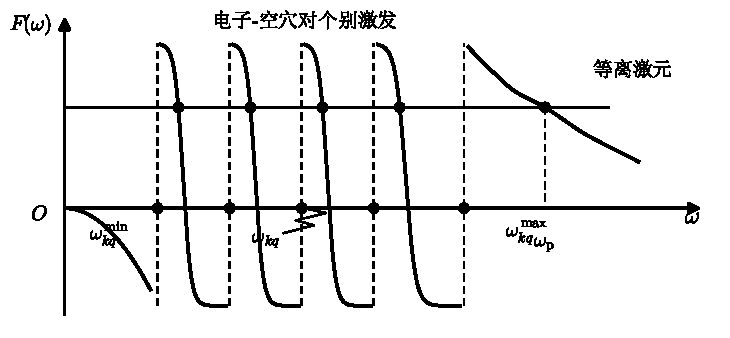
\includegraphics[width=10.5cm]{fig4-3.pdf}\\{\small 图 4.3\quad 确定 $q$ 值时电子系统的元激发 ($q<2k_{\mathrm{F}}$)}
\end{minipage}
\end{center}

这时 $\varepsilon$ 为复量，说明在此区域内不可能存在自发振荡.

对于 $\omega>\omega_{kq}^{\max}$ 的频率区域，式(4.7.2)存在另一支解，这是与 $\omega_{kq}$ 准连续解分离开的解.由于式(4.6.24)中 $\delta$ 函数的宗量在此频区内不可能等于零，故
\begin{equation}
  \mathrm{Im}\,\varepsilon(q,\omega)=\varepsilon_{2}(q,\omega)=0
  \quad\left(\omega>\omega_{kq}^{\max}\right)
\end{equation}
这时介电函数的虚部为零，说明振荡是无阻尼的.不难证明，这一支解代表电子气体的集体振荡.

\begin{center}
\begin{minipage}{4.5cm}
\centering
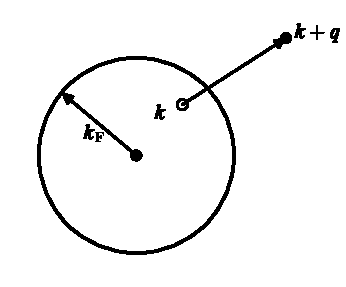
\includegraphics[width=4.5cm]{fig4-4.pdf}\\{\small 图 4.4\quad 电子-空穴对激发}
\end{minipage}
\end{center}

从 $\varepsilon_{1}(q,\omega)=0$ 出发，将式(4.7.2)按 $\left(\dfrac{\omega_{kq}}{\omega}\right)^{2}$ 展开
\begin{equation}
\begin{aligned}
  1=F(\omega)&=\frac{v(q)}{\hbar}\sum_{k}n_{k}
  \frac{4\omega_{kq}}{\omega^{2}-\omega_{kq}^{2}}\\
  &=\frac{v(q)}{\hbar}\sum_{k}n_{k}
  \bigg\{\frac{4\omega_{kq}}{\omega^{2}}+\frac{4\omega_{kq}^{3}}{\omega^{4}}+\cdots\bigg\}
\end{aligned}
\end{equation}
其中 $n_{k}$ 为零温度时费密分布 $2\displaystyle\sum_{k}n_{k}=N\ (n_{k}=n_{-k})$. 因此，准至 $\omega_{kq}$ 的展开式为
\begin{equation}
\begin{aligned}
  1\approx\frac{v(q)}{\hbar}\sum_{k}n_{k}\frac{4\omega_{kq}}{\omega^{2}}
  &=\frac{8\pi e^{2}}{q^{2}}\sum_{k}n_{k}\frac{1}{\omega^{2}}
  \Big(\frac{q^{2}}{m}+2\frac{\boldsymbol{q}\cdot\boldsymbol{k}}{m}\Big)\\
  &=\Big(\frac{4\pi e^{2}N}{m}\Big)\omega^{-2}
  =\Big(\frac{\omega_{\mathrm{p}}}{\omega}\Big)^{2}
\end{aligned}
\end{equation}
由此定出的解为
\begin{equation*}
  \omega\approx\left(\frac{4\pi e^{2}N}{m}\right)^{\frac{1}{2}}=\omega_{\mathrm{p}}
\end{equation*}
它正好就是 $q\to 0$ 时等离子振荡频率.若计及 $\omega_{kq}^{3}$ 项，利用对称性 $n_{k}=n_{-k}$ 可定出准至 $q^{2}$ 的等离子振荡频率
\begin{equation}
  \omega_{q}^{2}=\omega_{\mathrm{p}}^{2}+\frac{3}{5}q^{2}v_{\mathrm{F}}^{2}
  \quad\left(v_{\mathrm{F}}=\frac{\hbar k_{\mathrm{F}}}{m}\right)
\end{equation}
推导时还利用了 $k_{\mathrm{F}}^{3}=3\pi^{2}N$ 和 $n_{k}=\theta(k_{\mathrm{F}}-k)$.由式(4.7.7)求得等离激元的长波限色散关系为
\begin{equation}
  \omega_{q}=\omega_{\mathrm{p}}+\frac{3v_{\mathrm{F}}^{2}}{10\omega_{\mathrm{p}}}\,q^{2}
\end{equation}
当 $q\to 0$ 时，$\omega_{q}=\omega_{\mathrm{p}}\neq 0$，说明三维电子系统的等离子振荡元激发谱中存在相当大的能隙（约为10 eV），它不容易激发.

将个别激发区的边界
\begin{equation*}
\begin{aligned}
  \hbar\omega_{kq}^{\max}&=\frac{\hbar^{2}}{2m}\left(q^{2}+2k_{\mathrm{F}}q\right)\\
  \hbar\omega_{kq}^{\min}&=\left\{\begin{array}{ll}
  0 & (q<2k_{\mathrm{F}})\\[0.3em]
  \dfrac{\hbar^{2}}{2m}\left(q^{2}-2k_{\mathrm{F}}q\right) & (q\geqslant 2k_{\mathrm{F}})
  \end{array}\right.
\end{aligned}
\end{equation*}
和等离激元色散曲线式(4.7.8)在 $\omega$-$q$ 图上绘出，即是§1中的图4.2.图4.5是相同的图，但注明了各区域的 $\varepsilon_{2}$，便于讨论.由图4.5可以看出 $q=q_{c}$ 时集体激发与个别激发相交.当 $q<q_{c}$ 时等离激元的能量 $\hbar\omega_{q}$ 大于电子-空穴对的个别激发能量 $\hbar\omega_{kq}$，这时集体振荡的 $\mathrm{Im}\,\varepsilon=0$，等离激元不衰减为电子-空穴对，反之电子-空穴对也没有足够能量激发等离激元，两者彼此独立，但以集体激发为主.反之当 $q>q_{c}$ 时，由于 $\mathrm{Im}\,\varepsilon\neq 0$，等离子振荡不可能是稳定存在的自发振荡，这时只有个别对的激发.所以，只有在 $0<q<q_{c}$ 范围内才存在集体激发.因此，$q_{c}$ 是等离激元的波矢边界，它是划分个别与集体激发的一个重要参量.

\begin{center}
\begin{minipage}{5.5cm}
\centering
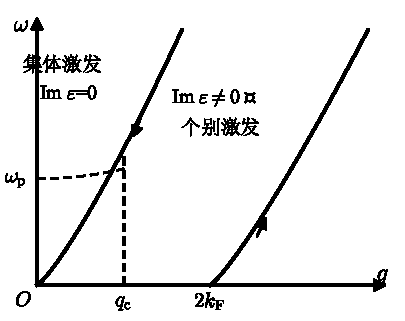
\includegraphics[width=5.5cm]{fig4-5.pdf}\\{\small 图 4.5}
\end{minipage}
\end{center}

比较个别激发和等离激元的色散关系可以估计 $q_{c}$ 的数值，若近似取 $\omega_{q}\approx\omega_{\mathrm{p}}$，则在交点处
\begin{equation*}
  \hbar\omega_{kq}^{\max}=\frac{\hbar^{2}q_{c}^{2}}{2m}
  +\frac{\hbar^{2}q_{c}k_{\mathrm{F}}}{m}
  \approx\hbar v_{\mathrm{F}}q_{c}=\hbar\omega_{\mathrm{p}}
\end{equation*}
可求得
\begin{equation*}
  q_{c}^{2}\approx\left(\frac{\omega_{\mathrm{p}}}{v_{\mathrm{F}}}\right)^{2}
  =\frac{4\pi e^{2}Nm}{\hbar^{2}k_{\mathrm{F}}^{2}}
  =\frac{2\pi Ne^{2}}{E_{\mathrm{F}}}
\end{equation*}
由此算出等离激元的总模数 $N_{\mathrm{p}}=\dfrac{1}{8\pi^{3}}\bigg(\dfrac{4\pi}{3}q_{c}^{3}\bigg)$ 与电子体系的总自由度 $3N$ 之比为
\begin{equation*}
  \frac{N_{\mathrm{p}}}{3N}=\frac{q_{c}^{3}}{6k_{\mathrm{F}}^{3}}
\end{equation*}
对于金属 Na，$\dfrac{N_{\mathrm{p}}}{3N}\approx 18\%$，存在于长波范围内.

金属中的等离子集体振荡是电子间库仑力导致的，由于库仑势场是纵场，因此等离激元是纵振动的量子.等离激元与等离子体不同，等离子体还有横向振荡，地球周围电离层能吸收电磁波就是由于等离子体的横向振荡被激发.

近年来由于人工制成了准二维电子系统（如液氦表面上的电子层和半导体中的 MOS 反型层），引起人们对二维电子体系的研究兴趣.可以利用本章求出的无规相近似介电函数公式计算二维电子体系等离激元的色散曲线，计算时应注意对于二维系统电子间库仑作用的傅里叶分量不再是 $\left(4\pi e^{2}/q^{2}\right)$，而是
\begin{equation}
  v_{\mathrm{2D}}(q)=\frac{2\pi e^{2}}{q}
\end{equation}
它仅与 $q^{-1}$ 成正比.将 $v_{\mathrm{2D}}(q)$ 代入式(4.7.5)，并对二维系统作类似式(4.7.6)、(4.7.7)的近似，可求得二维电子系统等离激元的长波色散关系
\begin{equation}
  \omega_{q}^{2}=\left(\frac{2\pi Ne^{2}}{m}\right)q+\frac{3}{4}q^{2}v_{\mathrm{F}}^{2}
\end{equation}
其中 $N$ 代表电子的面密度.显然
\begin{equation}
  \omega_{q}=\left(\frac{2\pi Ne^{2}}{m}\right)^{1/2}\sqrt{q}
  +o\left(q^{3/2}\right)
\end{equation}
与式(4.7.8)相比较可知二维系统的等离激元是无能隙的，它很容易激发，公式(4.7.11)已为实验所证实.

由于这类人造准二维系统的电子密度有相当大的调节范围，它给机理性研究提供了方便，并取得了较大的进展.例如，长期未观测到的维格纳晶格已在液氦表面的电子层中被证实\textsuperscript{[5]}.此外，半导体中还发现二维电子体系在强磁场作用下会出现分数量子霍尔效应等反常现象\textsuperscript{[6]}，从而为理论工作者提出了新的研究课题.

\section{静电屏蔽}

\subsection*{1. 屏蔽势}

静态外扰动属于介电函数的 $\omega=0$ 情况.根据式(4.6.24)，静态介电函数的虚部满足条件 $\mathrm{Im}\,\varepsilon(q,0)=0$，只有实部的贡献.因此，静态介电函数完全由式(4.6.23)决定：
\begin{equation}
\begin{aligned}
  \varepsilon(q,0)&=\mathrm{Re}\,\varepsilon(q,0)=\varepsilon_{1}(q,0)\\
  &=1+v(q)\sum_{k}\frac{4n_{k}}{\hbar\omega_{kq}}\\
  &=1+\frac{4\pi e^{2}}{q^{2}}\sum_{k<k_{\mathrm{F}}}
  \frac{4}{E_{k+q}-E_{k}}
\end{aligned}
\end{equation}
这个积分可直接算出
\begin{equation}
  \varepsilon_{1}(q,0)=1+\frac{4\pi e^{2}}{q^{2}}\,
  \frac{N}{\frac{2}{3}E_{\mathrm{F}}}
  \bigg\{\frac{1}{2}+\frac{4k_{\mathrm{F}}^{2}-q^{2}}{8k_{\mathrm{F}}q}
  \ln\bigg|\frac{2k_{\mathrm{F}}+q}{2k_{\mathrm{F}}-q}\bigg|\bigg\}
\end{equation}
其中 $E_{\mathrm{F}}$ 为费密能，先研究 $\varepsilon_{1}(q,0)$ 的长波情况；当 $q\ll 2k_{\mathrm{F}}$ 时，将上式对 $(q/2k_{\mathrm{F}})$ 作小量展开，得到介电函数的长波近似式
\begin{equation}
  \varepsilon_{1}(q,0)\approx 1+\left(\frac{6\pi Ne^{2}}{E_{\mathrm{F}}}\right)\frac{1}{q^{2}}
  \equiv 1+\frac{\lambda^{2}}{q^{2}}
\end{equation}
\begin{equation}
  \lambda^{2}=\frac{6\pi Ne^{2}}{E_{\mathrm{F}}}=3q_{c}^{2}
\end{equation}
式(4.8.3)称为托马斯-费密（Thomas-Fermi）介电函数.现在利用此近似式讨论原点处有一个 $(-e)$ 的电荷的屏蔽情况.这时，外扰动势的傅里叶分量为 $V_{\mathrm{e}}(q)=\dfrac{4\pi e^{2}}{q^{2}}=v(q)$，利用托马斯-费密介电函数和式(4.6.30)得到 $(V_{\mathrm{e}}/V)=\varepsilon$，可求总势能的傅里叶分量
\begin{equation}
  V_{\mathrm{TF}}(q)=\frac{V_{\mathrm{e}}(q)}{\varepsilon_{1}(q,0)}
  =\frac{4\pi e^{2}}{q^{2}+\lambda^{2}}
\end{equation}
而总势能的托马斯-费密公式为
\begin{equation}
  V_{\mathrm{TF}}(r)=\sum_{\boldsymbol{q}}\frac{4\pi e^{2}}{q^{2}+\lambda^{2}}
  \mathrm{e}^{\mathrm{i}\boldsymbol{q}\cdot\boldsymbol{r}}
  =\frac{e^{2}}{r}\,\mathrm{e}^{-\lambda r}
\end{equation}
上式表明，一个位于原点的 $(-e)$ 电荷将在 $\lambda^{-1}$ 距离内被屏蔽.由此不难推论，电子体系的屏蔽效应使金属中电子间的库仑互作用 $(e^{2}/r)$ 变为汤川（Yukawa）型互作用 $(e^{2}/r)\exp(-\lambda r)$，这里 $\lambda$ 与 $q_{c}$ 同量级，$q_{c}$ 是等离激元波数的上限.在玻姆-派因斯（Bohm-Pines）的早期理论中\textsuperscript{[7]}是从另一角度讨论屏蔽作用的.他们曾用幺正变换方法将库仑势傅里叶展开的长波部分 $(0<q<q_{c})$ 表示为等离子集体振荡，用于产生等离激元.这样，在库仑势中自然只剩下短波成分 $(q>q_{c})$，从而使个别电子间互作用成为短程屏蔽势.因为库仑作用的短波部分可写为
\begin{equation}
\begin{aligned}
  V_{\mathrm{SR}}(r)&=\sum_{q>q_{c}}\frac{4\pi e^{2}}{q^{2}}
  \mathrm{e}^{\mathrm{i}\boldsymbol{q}\cdot\boldsymbol{r}}
  =\frac{e^{2}}{2\pi}\int_{q>q_{c}}\frac{\mathrm{e}^{\mathrm{i}\boldsymbol{q}\cdot\boldsymbol{r}}}{q^{2}}\,\mathrm{d}^{3}q\\
  &=\frac{e^{2}}{r}\bigg\{1-\frac{2}{\pi}\int_{0}^{q_{c}r}
  \frac{\sin qr}{qr}\,\mathrm{d}(qr)\bigg\}\\
  &=\frac{e^{2}}{r}\bigg\{1-\frac{2}{\pi}\mathrm{Si}\left(q_{c}r\right)\bigg\}
\end{aligned}
\end{equation}
其中积分函数定义为
\begin{equation}
  \mathrm{Si}\left(q_{c}r\right)\equiv\int_{0}^{q_{c}r}\frac{\sin x}{x}\,\mathrm{d}x
\end{equation}
当 $q_{c}r\to\infty$ 时函数 $\mathrm{Si}(q_{c}r)\to\dfrac{\pi}{2}$，说明 $V_{\mathrm{SR}}$ 的作用局限在 $\left(1/q_{c}\right)$ 尺度之内，它和 $V_{\mathrm{TF}}$ 的屏蔽趋势基本相同.因此，扣除了集体振荡后，只剩下电子间的短程屏蔽互作用，好像在每个电子周围附加了一个半径约为 $\left(1/q_{c}\right)$ 的正电屏蔽壳层.从微观角度分析；由于关联效应，电子将排开周围电子，形成随电子运动的正电“空穴云”，施里弗（Schrieffer）称其为相关空穴，这种相关效应不仅表现为对电荷的屏蔽，还将产生运动学修正表现为改变电子的有效质量，并导致有限的寿命，我们将在§11中作专门的讨论.计及了这些修正的电子，实际上已经和多电子系统分不开了，只能认为是多体系统中的准粒子，这类准粒子被称为准电子.因此，我们应当把等离激元和准电子理解为互作用电子系统集体效应的两个方面.

\subsection*{2. 孔恩异常}

以上讨论的汤川型互作用只是式(4.8.2)取长波极限的近似公式.当研究晶体中杂质和缺陷对于电子和声子谱的影响时，往往需要更严格的公式，这时应当从式(4.8.2)出发，并将它改写为
\begin{equation}
  \left.\begin{aligned}
  \varepsilon_{1}(q,0)&=1+\frac{\lambda^{2}}{q^{2}}S\left(q/2k_{\mathrm{F}}\right)\\
  S(x)&\equiv\frac{1}{2}\bigg[1+\frac{1-x^{2}}{2x}
  \ln\bigg|\frac{1+x}{1-x}\bigg|\bigg]
  \end{aligned}\right\}
\end{equation}
当 $q\to 0$ 时 $S\to 1$，当 $q$ 很大时 $S\to 0$. 但在 $q=2k_{\mathrm{F}}$ 时，$\dfrac{\partial S}{\partial q}$ 发散，$S$ 函数有 $(q-2k_{\mathrm{F}})\ln\left(q-2k_{\mathrm{F}}\right)$ 型的对数奇性.图4.6是屏蔽参数 $\lambda^{2}S$ 随 $q$ 的变化曲线，静态介电函数在 $q=2k_{\mathrm{F}}$ 点也有相似变化.屏蔽参数及介电函数在 $q=2k_{\mathrm{F}}$ 处的突然下降是由于电子气的基态分布在费密能量上有不连续性，而费密球的直径恰好为 $2k_{\mathrm{F}}$. 更具体的说明如下：

比较式(4.8.1)和(4.8.9)有
\begin{equation}
  \lambda^{2}S\left(q/2k_{\mathrm{F}}\right)=4v(q)q^{2}
  \sum_{k<k_{\mathrm{F}}}\frac{1}{\left(E_{k+q}-E_{k}\right)}
\end{equation}
显然，$\lambda^{2}S$ 的大小与能量分母 $\left(E_{k+q}-E_{k}\right)$ 有关，这里 $\boldsymbol{k}$ 为费密球内已被占据态，只要 $|\boldsymbol{q}|<2k_{\mathrm{F}}$，我们总可以作出一个矢量 $\boldsymbol{q}$，使 $\boldsymbol{k}$ 与 $\boldsymbol{k}+\boldsymbol{q}$ 都落在费密面附近，因此式(4.8.10)中总有一些项的能量分母较小.所以，当 $|\boldsymbol{q}|<2k_{\mathrm{F}}$ 时，$\lambda^{2}S$ 和 $\varepsilon$ 都比较大.但是，当 $|\boldsymbol{q}|\geqslant 2k_{\mathrm{F}}$ 时，由于 $|\boldsymbol{q}|$ 已超过费密球直径 $2k_{\mathrm{F}}$，上述可能性消失，式(4.8.10)中各项的能量分母都比较大，因此，在 $q=2k_{\mathrm{F}}$ 处屏蔽参数和介电函数将突然下降.

\begin{center}
\begin{minipage}{5cm}
\centering
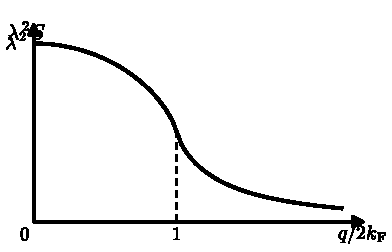
\includegraphics[width=5cm]{fig4-6.pdf}\\{\small 图 4.6}
\end{minipage}
\end{center}

介电函数和在 $q=2k_{\mathrm{F}}$ 点的奇性，对于声子谱有重要影响.金属晶格中离子的振动可看作电子的一个扰动势场，而电子对此扰动场的响应又将反过来屏蔽离子势，使离子间有效互作用减弱，并导致晶格振动频率下降.因此，介电函数在 $2k_{\mathrm{F}}$ 处的奇性也必然会反映在声子的 $\omega(q)$ 曲线上.实验已观察到，在三维金属 Pb 中 $q=2k_{\mathrm{F}}$ 的声子频率有软化现象，并称之为孔恩异常（Kohn anomalies）.近年来又发现，在链状固体 KCP 和 TTF-TCNQ 中，当温度趋于某临界值时，$2k_{\mathrm{F}}$ 声子频率将突然下降到很小的数值（接近零）\textsuperscript{[8]}.这种 $2k_{\mathrm{F}}$ 声子的完全软化现象称为强孔恩异常，它是一维系统中电子元激发特征的反映.一维系统的电子-空穴对激发区与二维或三维系统有本质区别，其个别对激发 $\hbar\omega_{kq}=E_{k+q}-E_{k}\ (|k|<k_{\mathrm{F}},\,|k+q|>k_{\mathrm{F}})$ 仅在图4.7的（Ⅰ）区中出现.（Ⅱ）区中不存在 $\omega_{kq}$ 激发，是一维系统个别激发的空隙区.因此，一维系的声子色散曲线（Ⅲ）只能在 $2k_{\mathrm{F}}$ 附近与电子系统的个别激发谱相交，这时费密面上的电子将通过 $k_{\mathrm{F}}\to(-k_{\mathrm{F}})$ 的对端跃迁吸收或发射 $2k_{\mathrm{F}}$ 声子，使声子谱中 $2k_{\mathrm{F}}$ 波矢附近的晶格离子振动受到电子系统的强烈屏蔽，并产生 $2k_{\mathrm{F}}$ 声子的明显软化效应，这就是链状固体中出现强孔恩异常的物理实质.

\begin{center}
\begin{minipage}{6cm}
\centering
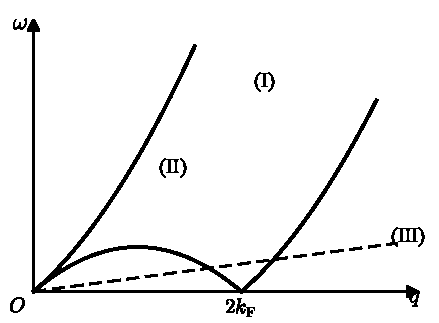
\includegraphics[width=6cm]{fig4-7.pdf}\\{\small 图 4.7\quad 一维系中电子与声子谱的共振特征}\\[0.2em]
{\small （Ⅰ）电子-空穴对激发区；（Ⅱ）个别激发的空隙区；（Ⅲ）声子色散曲线}
\end{minipage}
\end{center}

\subsection*{3. 夫里德耳振荡}

现在利用静态介电函数讨论金属中电子对杂质（或点缺陷）的屏蔽作用.设杂质位于原点并带有 $Ze$ 电荷，则杂质受电子体系屏蔽的有效势能为
\begin{equation}
  V(\boldsymbol{r})=-\sum_{\boldsymbol{q}}
  \frac{4\pi Ze^{2}}{\varepsilon_{1}(q,0)\,q^{2}}
  \mathrm{e}^{\mathrm{i}\boldsymbol{q}\cdot\boldsymbol{r}}
\end{equation}
将严格公式(4.8.9)代入上式得
\begin{equation}
  V(\boldsymbol{r})=-\frac{1}{8\pi^{3}}\int
  \frac{4\pi Ze^{2}}{q^{2}+\lambda^{2}S\left(q/2k_{\mathrm{F}}\right)}
  \mathrm{e}^{\mathrm{i}\boldsymbol{q}\cdot\boldsymbol{r}}\,\mathrm{d}^{3}q
\end{equation}
这个积分可用近似方法计算\textsuperscript{[9]}，在 $r$ 很大时有渐近式
\begin{equation}
  V(r)\sim\frac{\cos 2k_{\mathrm{F}}r}{r^{3}}
\end{equation}
上式代表一个以 $2k_{\mathrm{F}}$ 为波数的振荡势能，称为夫里德耳（Friedel）振荡势.图4.8对夫里德耳振荡势和汤川势型屏蔽势作了比较，两者有相同的屏蔽趋势，但差别在于长程振荡.

\begin{center}
\begin{minipage}{5.5cm}
\centering
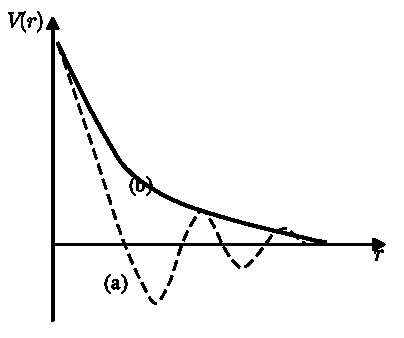
\includegraphics[width=5.5cm]{fig4-8.pdf}\\{\small 图 4.8\quad (a) 夫里德耳振荡势；(b) 汤川势}
\end{minipage}
\end{center}

再看杂质周围屏蔽电子数密度 $\Delta\rho(r)$ 的空间分布，从泊松方程出发
\begin{equation}
  \nabla^{2}V(r)=4\pi e^{2}\left\{Z\delta(r)-\Delta\rho(r)\right\}
\end{equation}
将 $V(r)$ 的严格式(4.8.11)代入，求得
\begin{equation}
  \Delta\rho(\boldsymbol{r})=\frac{Z}{8\pi^{3}}\int
  \left(1-\frac{1}{\varepsilon_{1}(q,0)}\right)
  \mathrm{e}^{\mathrm{i}\boldsymbol{q}\cdot\boldsymbol{r}}\,\mathrm{d}^{3}q
\end{equation}
当 $r\to\infty$ 时，$\Delta\rho$ 的渐近式为
\begin{equation}
  \Delta\rho(r)\sim\frac{\cos 2k_{\mathrm{F}}r}{r^{3}}
\end{equation}
说明在杂质周围屏蔽电荷的分布也具有长程振荡特征，这就是著名的夫里德耳振荡.如果用汤川势代入泊松方程，则 $\Delta\rho$ 变为
\begin{equation}
  \Delta\rho(r)\sim\frac{Z\lambda^{2}}{4\pi}\,\frac{\mathrm{e}^{-\lambda r}}{r}
\end{equation}
与式(4.8.16)相比较，屏蔽电荷失去了长程振荡特性，这是因为汤川势来源于对 $S\left(q/2k_{\mathrm{F}}\right)$ 取长波近似，它只是准经典理论的结果，实际上不能充分反映电子系统的量子效应.

产生夫里德耳振荡的原因主要是由于金属中电子有明确的费密面.正如前面讨论孔恩异常时的分析，由于 $T=0$ K 时电子分布严格限制在 $|k|=k_{\mathrm{F}}$ 球内，静态介电函数 $\varepsilon_{1}(q,0)$ 将在 $q=2k_{\mathrm{F}}$ 处有突然下降，$\varepsilon_{1}(q,0)$ 的这个奇异性使积分式(4.8.15)的主要贡献来源于 $q=2k_{\mathrm{F}}$ 项，从而得到 $\Delta\rho$ 与 $V(r)$ 都以 $2k_{\mathrm{F}}$ 波数振荡的结果.从物理观点分析，金属中参加屏蔽的粒子主要是费密面上的电子，由于这些电子的德布罗意波在杂质上的衍射效应，使围绕杂质的屏蔽电荷分布起振荡变化，从而形成与小孔衍射光圈图相似的 $\Delta\rho(r)$ 分布图案.夫里德耳指出\textsuperscript{[10]}，这时在杂质周围不是形成一个（或两个）电子的束缚态，而是费密面上电子在杂质势阱中形成共振态并具有有限寿命.关于共振散射态理论，我们将在第十一章中讨论局域磁矩时用格林函数方法作介绍，其初级理论可参阅有关量子力学书籍（例如第一章文献[3]p235）.

\section{基态能}

互作用电子体系的基态能直接关系到金属结合能的定量估计，是固体理论的重要问题.但是，过去基态能只有哈特利-福克近似（HFA）的计算结果，进一步的微扰修正，由于涉及长程库仑力，遇到了发散困难.直到等离激元理论问世以后，人们才认识到应当在集体振荡的基础上用屏蔽库仑势作计算，从而克服了库仑势长程部分带来的发散困难，使基态能的研究进入定量计算阶段.本节首先介绍基态能的哈特利-福克近似计算及其存在的困难，然后再利用介电函数导出基态能的严格公式，并给出高密度电子体系基态能的计算结果.

\subsection*{1. 哈特利-福克近似的基态能}

对于互作用电子体系哈密顿量
\begin{equation}
  H=H_{0}+H'=\sum_{k,\sigma}\frac{\hbar^{2}k^{2}}{2m}C_{k\sigma}^{+}C_{k\sigma}
  +\frac{1}{2}\mathop{{\sum}'}\limits_{q}v(q)\left(\rho_{q}^{+}\rho_{q}-N\right)
\end{equation}
的一阶微扰计算叫哈特利-福克近似.因此，在哈特利-福克近似范围内只需用无相互作用电子系的基态（费密球状态）
\begin{equation}
  |0\rangle_{0}=\prod_{k\sigma}C_{k\sigma}^{+}\ |\ \mathrm{Vac}\rangle
\end{equation}
对 $H$ 求对角平均.其中 $|\mathrm{Vac}\rangle$ 代表 $k$ 空间全部未被占据的状态，即真正的真空态.

哈特利-福克近似的基态能
\begin{equation}
  E_{0}\left(\mathrm{HFA}\right)=E_{k}+E_{\mathrm{ex}}
\end{equation}
其中
\begin{equation}
\begin{aligned}
  E_{\mathrm{K}}={}_{0}\langle 0|H_{0}|0\rangle_{0}
  &=\sum_{k,\sigma}\frac{\hbar^{2}k^{2}}{2m}\,
  {}_{0}\langle 0|C_{k\sigma}^{+}C_{k\sigma}|0\rangle_{0}\\
  &=2\sum_{k}\frac{\hbar^{2}k^{2}}{2m}\theta\left(k_{\mathrm{F}}-k\right)
  =\frac{3}{5}NE_{\mathrm{F}}
\end{aligned}
\end{equation}
代表电子体系的总动能，$E_{\mathrm{F}}=\left(\hbar^{2}k_{\mathrm{F}}^{2}/2m\right)$ 为费密能，而
\begin{equation}
\begin{aligned}
  E_{\mathrm{ex}}&={}_{0}\langle 0|H'|0\rangle_{0}
  =\frac{1}{2}\mathop{{\sum}'}\limits_{q}v(q)
  \left({}_{0}\langle 0|\rho_{q}^{+}\rho_{q}|0\rangle_{0}-N\right)\\
  &=\frac{1}{2}\mathop{{\sum}'}\limits_{q}v(q)\sum_{k_{1},k_{2}}\sum_{\sigma_{1},\sigma_{2}}
  {}_{0}\langle 0|C_{k_{1}+q,\sigma_{1}}^{+}C_{k_{2}-q,\sigma_{2}}^{+}
  C_{k_{2}\sigma_{2}}C_{k_{1}\sigma_{1}}|0\rangle_{0}\\
  &=-\sum_{k_{1}}\sum_{k_{2}}
  \frac{4\pi e^{2}}{|k_{1}-k_{2}|^{2}}
  \theta\left(k_{\mathrm{F}}-k_{1}\right)\theta\left(k_{\mathrm{F}}-k_{2}\right)
\end{aligned}
\end{equation}
由于 $q\neq 0$，因此在上式中只有 $\boldsymbol{k}_{2}=\boldsymbol{k}_{1}+\boldsymbol{q}$，$\sigma_{2}=\sigma_{1}$ 项的贡献，它代表自旋平行电子之间的交换能.式(4.9.5)的计算是直截了当的，可令
\begin{equation}
  E_{\mathrm{ex}}=\sum_{k_{1}}\theta\left(k_{\mathrm{F}}-k_{1}\right)
  \mathcal{E}_{\mathrm{ex}}\left(k_{1}\right)
\end{equation}
这里 $\mathcal{E}_{\mathrm{ex}}$ 是单电子的自能修正
\begin{equation}
\begin{aligned}
  \mathcal{E}_{\mathrm{ex}}(\boldsymbol{k}_{1})
  &=-\sum_{k_{2}}\frac{4\pi e^{2}}{|\boldsymbol{k}_{1}-\boldsymbol{k}_{2}|^{2}}
  \theta\left(k_{\mathrm{F}}-k_{2}\right)\\
  &=\frac{e^{2}}{\pi}\int_{0}^{k_{\mathrm{F}}}k_{2}^{2}\,\mathrm{d}k_{2}
  \int_{-1}^{1}\frac{\mathrm{d}\mu}{k_{1}^{2}+k_{2}^{2}-2k_{1}k_{2}\mu}
  =-\frac{2e^{2}}{\pi}k_{\mathrm{F}}S(x)
\end{aligned}
\end{equation}
其中 $x\equiv\left(k_{1}/k_{\mathrm{F}}\right)$
\begin{equation}
  S(x)=\frac{1}{2}\bigg\{1+\frac{1-x^{2}}{2x}
  \ln\bigg|\frac{1+x}{1-x}\bigg|\bigg\}
\end{equation}
代入式(4.9.6)，再将 $\boldsymbol{k}_{1}$ 求和化为积分，算出交换能
\begin{equation}
\begin{aligned}
  E_{\mathrm{ex}}&=-\frac{2e^{2}}{\pi}k_{\mathrm{F}}^{4}\,\frac{1}{8\pi^{3}}
  \int S(x)\,\mathrm{d}^{3}x\\
  &=-\bigg(\frac{3e^{2}}{\pi}k_{\mathrm{F}}\bigg)N\int_{0}^{1}x^{2}S(x)\,\mathrm{d}x\\
  &=-N\bigg(\frac{3e^{2}}{4\pi}\bigg)k_{\mathrm{F}}
\end{aligned}
\end{equation}
其中利用了关系式 $k_{\mathrm{F}}^{3}=3\pi^{2}N$ 和 $S(x)$ 的下列定积分
\begin{equation}
  4\int_{0}^{1}x^{2}S(x)\,\mathrm{d}x=1
\end{equation}
因此，在哈特利-福克近似中平均每个电子的基态能量为
\begin{equation}
  \frac{1}{N}E_{0}\left(\mathrm{HFA}\right)
  =\frac{3}{5}\,\frac{\hbar^{2}k_{\mathrm{F}}^{2}}{2m}
  -\frac{3e^{2}}{4\pi}k_{\mathrm{F}}
\end{equation}
讨论电子体系基态能时常采用量纲为 1 的参量 $r_{s}$ 描述系统的电子密度，其定义为
\begin{equation}
  N\,\frac{4\pi}{3}\left(r_{s}a_{\mathrm{H}}\right)^{3}=1
\end{equation}
其中 $a_{\mathrm{H}}=\dfrac{\hbar^{2}}{me^{2}}$ 是氢原子的第一玻尔轨道半径.由上式可知，$r_{s}a_{\mathrm{H}}$ 代表平均一个电子所占球体之半径，当 $r_{s}<1$ 时称为高密度电子气，反之当 $r_{s}\gg 1$ 属于低密度情况.用 $r_{s}$ 表示的费密波数为
\begin{equation}
  k_{\mathrm{F}}=\left(\frac{9\pi}{4}\right)^{1/3}
  \frac{1}{r_{s}a_{\mathrm{H}}}
\end{equation}
将式(4.9.13)代入式(4.9.11)求得哈特利-福克近似的基态能
\begin{equation}
  \frac{1}{N}E_{0}\left(\mathrm{HFA}\right)
  =\frac{2.21}{r_{s}^{2}}-\frac{0.916}{r_{s}}\quad\left[\mathrm{Ry}\right]
\end{equation}
其中能量用里德伯单位［Ry］
\begin{equation}
  1\ \left[\mathrm{Ry}\right]\equiv\frac{me^{4}}{2\hbar^{2}}
  =\frac{e^{2}}{2a_{\mathrm{H}}}=13.6\ \mathrm{eV}
\end{equation}
上述哈特利-福克近似结果可以定性说明系统的结合，但算出的结合能定量数值明显偏小.例如金属锂（Li）结合能的实验值为 36.5［Ry］而哈特利-福克近似的计算值仅为 17［Ry］.为了改进计算结果，人们曾经尝试计算库仑作用的二阶以及高阶微扰修正，但是都碰到了发散困难.

\subsection*{2. 相关能的二阶微扰计算}

在哈特利-福克近似基础上，计入反平行自旋电子间库仑作用所降低的能量称为相关能，最低阶的相关能可利用二阶微扰公式
\begin{equation}
  E^{(2)}=-\mathop{{\sum}'}\limits_{n}
  \frac{\left|\,{}_{0}\langle 0|H'|n\rangle_{0}\right|^{2}}{E_{n}-E_{0}}
\end{equation}
求出，其中 $|n\rangle_{0}$ 为中间态，求和的限制是 $E_{n}\neq E_{0}$. 先讨论一对 $\boldsymbol{k}_{1}\uparrow$ 与 $\boldsymbol{k}_{2}\downarrow$ 电子经 $H'$ 散射到中间态 $\boldsymbol{k}_{3}\uparrow$ 与 $\boldsymbol{k}_{4}\downarrow$，并将初态 $|0\rangle_{0}$ 记为 $|12\rangle$，而中间态则用 $|34\rangle$ 表示.根据泡利原理，$\boldsymbol{k}_{1}$ 与 $\boldsymbol{k}_{2}$ 必须位于费密球内，而 $\boldsymbol{k}_{3}$ 与 $\boldsymbol{k}_{4}$ 均应在球外，这时 1 与 2 电子之间的直接互作用项为
\begin{equation}
  E_{\mathrm{c}}^{(2)}\left(k_{1},k_{2}\right)
  =-\left(\frac{2m}{\hbar^{2}}\right)\sum_{k_{3}}\sum_{k_{4}}
  \frac{\langle 12|H'|34\rangle\langle 34|H'|12\rangle}
  {\left[\left(k_{3}^{2}+k_{4}^{2}\right)-\left(k_{1}^{2}+k_{2}^{2}\right)\right]}
  \left(1-n_{k_{3}}\right)\left(1-n_{k_{4}}\right)
\end{equation}
其中 $n_{k_{3}}=\theta\left(k_{\mathrm{F}}-k_{3}\right)$，$\left(1-n_{k_{3}}\right)\left(1-n_{k_{4}}\right)$ 因子的出现保证了 $\boldsymbol{k}_{3}$ 与 $\boldsymbol{k}_{4}$ 电子均在费密球外.当取体积 $V=1$ 时，微扰矩阵元为
\begin{equation}
  \langle 34|H'|12\rangle=\frac{4\pi e^{2}}{q^{2}}\,
  \delta_{\boldsymbol{k}_{1}+\boldsymbol{k}_{2},\,\boldsymbol{k}_{3}+\boldsymbol{k}_{4}}
\end{equation}
散射的动量守恒条件可用波矢 $\boldsymbol{q}$ 的下列等式表示
\begin{equation}
  \boldsymbol{q}\equiv\boldsymbol{k}_{1}-\boldsymbol{k}_{3}
  =\boldsymbol{k}_{4}-\boldsymbol{k}_{2}
\end{equation}
从而得到 $\boldsymbol{k}_{3}=\boldsymbol{k}_{1}-\boldsymbol{q}$ 与 $\boldsymbol{k}_{4}=\boldsymbol{k}_{2}+\boldsymbol{q}$.由于 $\boldsymbol{k}_{3}$ 与 $\boldsymbol{k}_{4}$ 并不独立，可改用波矢 $\boldsymbol{q}$，将式(4.9.17)改写为
\begin{equation}
  E_{\mathrm{c}}^{(2)}\left(k_{1},k_{2}\right)
  =-\left(\frac{2m}{\hbar^{2}}\right)\mathop{{\sum}'}\limits_{q}
  \left(\frac{4\pi e^{2}}{q^{2}}\right)^{2}
  \frac{\left(1-n_{k_{1}-q}\right)\left(1-n_{k_{2}+q}\right)}
  {\left[q^{2}+q\cdot\left(k_{2}-k_{1}+q\right)\right]}
\end{equation}
上式对 $\boldsymbol{k}_{1}$ 与 $\boldsymbol{k}_{2}$ 求和后，得到总的二阶修正
\begin{equation}
\begin{aligned}
  E_{\mathrm{c}}^{(2)}&=\sum_{k_{1}}\sum_{k_{2}}E_{\mathrm{c}}^{(2)}\left(k_{1},k_{2}\right)\\
  &=-\sum_{k_{1},k_{2}}\mathop{{\sum}'}\limits_{q}
  \left(\frac{2m}{\hbar^{2}}\right)\left(\frac{4\pi e^{2}}{q^{2}}\right)^{2}
  \frac{n_{k_{1}}\left(1-n_{k_{1}-q}\right)\left(1-n_{k_{2}+q}\right)}
  {\left[q^{2}+q\cdot\left(k_{2}-k_{1}+q\right)\right]}
\end{aligned}
\end{equation}
为了便于运算和将 $E_{\mathrm{c}}^{(2)}$ 用里德伯单位 $\left(e^{2}/2a_{\mathrm{H}}\right)$ 量度，作下列变量代换：
\begin{equation}
  \boldsymbol{k}_{1}\to-\boldsymbol{p}k_{\mathrm{F}},\quad
  \boldsymbol{k}_{2}\to\boldsymbol{k}k_{\mathrm{F}},\quad
  \boldsymbol{q}\to\boldsymbol{q}k_{\mathrm{F}}
\end{equation}
使所有波矢的量纲均为 1，再考虑到系统为各向同性时 $\boldsymbol{n}_{-p}=\boldsymbol{n}_{p}=\theta\left(1-p\right)$，可将相关能的修正写为
\begin{equation}
  E_{\mathrm{c}}^{(2)}=\left(\frac{Ne^{2}}{2a_{\mathrm{H}}}\right)
  \varepsilon_{\mathrm{c}}^{(2)}
\end{equation}
其中
\begin{equation}
  \varepsilon_{\mathrm{c}}^{(2)}=-\left(\frac{3}{8\pi^{5}}\right)
  \int\frac{\mathrm{d}^{3}q}{q^{4}}\,f(\boldsymbol{q})
\end{equation}
\begin{equation}
  f(\boldsymbol{q})=\int\mathrm{d}^{3}p\int\mathrm{d}^{3}k\,
  \frac{\theta\left(1-p\right)\left[1-\theta\left(1-|\boldsymbol{p}+\boldsymbol{q}|\right)\right]
  \theta\left(1-k\right)\left[1-\theta\left(1-|\boldsymbol{k}+\boldsymbol{q}|\right)\right]}
  {\left[q^{2}+\boldsymbol{q}\cdot\left(\boldsymbol{p}+\boldsymbol{k}+\boldsymbol{q}\right)\right]}
\end{equation}
$\varepsilon_{\mathrm{c}}^{(2)}$ 代表在里德伯单位中平均每个格点的二阶修正能量.显然，对 $\varepsilon_{\mathrm{c}}^{(2)}$ 的主要贡献来自长波 $(q\to 0)$ 部分.为此，先作长波近似，讨论 $q\to 0$ 时 $\varepsilon_{\mathrm{c}}^{(2)}$ 的渐近行为.当 $\boldsymbol{q}\to 0$ 时，阶跃函数中的 $q^{2}$ 项可略去，有长波近似式
\begin{equation}
  \theta\left(1-|\boldsymbol{p}+\boldsymbol{q}|\right)=\theta\left(1-p\right)
  -\left(\boldsymbol{q}\cdot\boldsymbol{p}/p\right)\delta\left(1-p\right)
\end{equation}
由此求得在长波近似下泡利原理对 $\boldsymbol{p}$ 电子激发的一个限制
\begin{subequations}
\begin{equation}
\begin{aligned}
  \theta\left(1-p\right)\left[1-\theta\left(|\boldsymbol{p}+\boldsymbol{q}|\right)\right]
  &=\theta\left(1-p\right)\left\{\left[1-\theta\left(1-p\right)\right]
  +\left(\boldsymbol{q}\cdot\boldsymbol{p}/p\right)\delta\left(1-p\right)\right\}\\
  &=\theta\left(1-p\right)\delta\left(1-p\right)
  \left(\boldsymbol{q}\cdot\boldsymbol{p}/p\right)\geqslant 0
\end{aligned}
\end{equation}
其中利用了阶跃函数的 $\theta(x)\left[1-\theta(x)\right]=0$ 特征.上式在物理上表明，在长波近似下互作用激发的电子仅限于费密面 $(p=1)$ 附近极薄的壳层内，其厚度正比于 $\boldsymbol{q}$. 此外，上式还限定 $\boldsymbol{p}\cdot\boldsymbol{q}\geqslant 0$，此即要求 $\boldsymbol{p}$ 与 $\boldsymbol{q}$ 间的夹角余弦 $y=\cos\theta_{pq}\geqslant 0$，此限制也可从泡利原理所要求的 $p\leqslant 1$ 和 $|\boldsymbol{p}+\boldsymbol{q}|\geqslant 1$，在长波近似下略去 $q^{2}$ 项后直接导出.因此，在长波近似下，泡利原理对 $\boldsymbol{p}$ 电子激发的另一限制是
\begin{equation}
  0\leqslant y\leqslant 1
\end{equation}
\end{subequations}
对于 $k$ 电子，也存在相同的限制，这时可将 $f(\boldsymbol{q})$ 表示式分母中 $q^{2}$ 项略去，积分后求得
\begin{subequations}
\begin{equation}
  \lim_{q\to 0}f(\boldsymbol{q})=(2\pi)^{2}Iq
\end{equation}
其中
\begin{equation}
  I\equiv\int_{0}^{1}\mathrm{d}y\int_{0}^{1}\mathrm{d}z\,
  \frac{yz}{y+z}=\frac{2}{3}\left(1-\ln 2\right)
\end{equation}
\end{subequations}
这样就求出了相关能 $\varepsilon_{\mathrm{c}}^{(2)}$ 的长波特性
\begin{equation}
  \lim_{q\to 0}\varepsilon_{\mathrm{c}}^{(2)}
  =-\bigg(\frac{4}{\pi^{2}}\bigg)\left(1-\ln 2\right)\int\frac{\mathrm{d}q}{q}
  \sim-\ln q
\end{equation}
显然，当 $q\to 0$ 时 $\varepsilon_{\mathrm{c}}^{(2)}$ 呈现对数式发散.但是，在大 $\boldsymbol{q}$ 情况下 $(q\gg 2k_{\mathrm{F}}$ 时$)$，由于式(4.9.25)分母中 $\boldsymbol{q}\cdot(\boldsymbol{p}+\boldsymbol{k})$ 项可略去，并且当 $q>2k_{\mathrm{F}}$ 时，总有 $\theta\left(1-|\boldsymbol{p}+\boldsymbol{q}|\right)=0$ 和 $\theta\left(1-|\boldsymbol{k}+\boldsymbol{q}|\right)=0$，将使 $f(\boldsymbol{q})$ 的积分简化为
\begin{subequations}
\begin{equation}
  \lim_{q\to\infty}f(q)=\int\mathrm{d}^{3}p\int\mathrm{d}^{3}k\,
  \theta\left(1-p\right)\theta\left(1-k\right)
  =\left(\frac{4\pi}{3}\right)^{2}/q^{2}
\end{equation}
由此求出 $\varepsilon_{\mathrm{c}}^{(2)}$ 在 $q\to\infty$ 时的特征为
\begin{equation}
  \lim_{q\to\infty}\varepsilon_{\mathrm{c}}^{(2)}
  =-\frac{3}{8\pi^{5}}\int\mathrm{d}^{3}q\;q^{-4}\lim_{q\to\infty}f(q)
  =\frac{8}{3\pi^{2}}\,q^{-3}
\end{equation}
\end{subequations}
它按照 $\boldsymbol{q}^{-3}$ 趋于零，是收敛的.

根据以上讨论可知，用微扰论计算相关能的主要困难来自长波部分存在 ln $q$ 型的对数式发散.类似的长波发散还出现在三阶以至所有高阶的微扰计算之中，这是建立金属基态能理论的主要困难.

微扰理论之所以产生相关能发散的困难是因为没有考虑互作用对电子态的影响（即多体效应）\nobreak.因此，为了消除发散，必须在集体运动的基础上考虑屏蔽效应，下面将从多体系统的介电函数理论出发，推导基态能的严格公式.

\subsection*{3. 基态能的严格公式——费因曼定理}

利用附录B中严格介电函数公式(B.14)
\begin{equation}
  \mathrm{Im}\bigg[\frac{1}{\varepsilon(q,\omega)}\bigg]
  =\frac{\pi v(q)}{\hbar}\sum_{n}
  |\langle n|\rho_{q}|0\rangle|^{2}
  \left[\delta\left(\omega+\omega_{n0}\right)-\delta\left(\omega-\omega_{n0}\right)\right]
\end{equation}
其中
\begin{equation}
  \omega_{n0}\equiv\frac{1}{\hbar}\left(\mathcal{E}_{n}-\mathcal{E}_{0}\right)
\end{equation}
$|n\rangle$ 和 $\mathcal{E}_{n}$ 为多体系 $H$ 的严格本征态和能量本征值，$|0\rangle$ 代表严格基态.

利用 $\mathrm{Im}\bigg[\dfrac{1}{\varepsilon(q,\omega)}\bigg]$ 既可以计算库仑相互作用能量，也能求出互作用电子系统的基态能量.

式(4.9.31)对 $\omega$ 积分，考虑到 $\omega_{n0}>0$，应有
\begin{equation}
\begin{aligned}
  \int_{0}^{\infty}\mathrm{d}\omega\,
  \mathrm{Im}\bigg[\frac{1}{\varepsilon(q,\omega)}\bigg]
  &=-\frac{4\pi^{2}e^{2}}{q^{2}\hbar}\sum_{n}
  |\langle n|\rho_{q}|0\rangle|^{2}\\
  &=-\frac{\pi v(q)}{\hbar}\langle 0|\rho_{q}^{+}\rho_{q}|0\rangle
\end{aligned}
\end{equation}
由于电子间库仑互作用
\begin{equation}
  H'=\frac{1}{2}\mathop{{\sum}'}\limits_{q}v(q)
  \left(\rho_{q}^{+}\rho_{q}-N\right)
\end{equation}
利用公式(4.9.33)可求得 $H'$ 对严格基态的平均
\begin{equation}
  \langle 0|H'|0\rangle=-\mathop{{\sum}'}\limits_{q}
  \bigg\{\frac{\hbar}{2\pi}\int_{0}^{\infty}\mathrm{d}\omega\,
  \mathrm{Im}\bigg[\frac{1}{\varepsilon(q,\omega)}\bigg]
  +\frac{1}{2}v(q)N\bigg\}
\end{equation}
这是库仑能与介电函数的严格关系式.

现在推导基态能 $\langle 0|H|0\rangle$ 与介电函数的关系式.为了计算基态能还必须求动能部分
\begin{equation}
  H_{0}=\sum_{k,\sigma}E_{k}C_{k\sigma}^{+}C_{k\sigma}
\end{equation}
对严格基态的平均 $\langle 0|H_{0}|0\rangle$，由于存在库仑作用，零温度时的平均动能不再等于无相互作用电子系统的基态能 $E_{0}(0)=\dfrac{3}{5}NE_{\mathrm{F}}$，而且平均动能 $\langle 0|H_{0}|0\rangle$ 又不像库仑能 $\langle 0|H'|0\rangle$ 与介电函数直接有关.这时必须应用费因曼定理才能求得基态能量 $E_{0}=\langle 0|H|0\rangle$ 与介电函数的关系式.

费因曼（Feynman）定理：设互作用系统的哈密顿量与可调参数 $\lambda$ 有关，并记为 $H(\lambda)$，则对应于态 $\psi_{n}(\lambda)$ 的能量本征值
\begin{equation}
  E_{n}(\lambda)=\langle\psi_{n}(\lambda)|H(\lambda)|\psi_{n}(\lambda)\rangle
\end{equation}
满足关系式
\begin{equation}
  \frac{\partial E_{n}(\lambda)}{\partial\lambda}
  =\bigg\langle\psi_{n}(\lambda)\bigg|
  \frac{\partial H(\lambda)}{\partial\lambda}\bigg|\psi_{n}(\lambda)\bigg\rangle
\end{equation}
其中波函数是归一的
\begin{equation}
  \langle\psi_{n}(\lambda)|\psi_{n}(\lambda)\rangle=1
\end{equation}
式(4.9.38)称为费因曼定理，它是计算互作用系统基态能和自由能的一个重要工具，在格林函数理论中被广泛应用.

证明过程如下：对式(4.9.37)求导得
\begin{equation}
\begin{aligned}
  \frac{\partial E_{n}(\lambda)}{\partial\lambda}
  ={}&\bigg\langle\psi_{n}(\lambda)\bigg|
  \frac{\partial H(\lambda)}{\partial\lambda}\bigg|\psi_{n}(\lambda)\bigg\rangle\\
  &+\bigg\langle\frac{\partial\psi_{n}(\lambda)}{\partial\lambda}
  \bigg|H(\lambda)\bigg|\psi_{n}(\lambda)\bigg\rangle
  +\bigg\langle\psi_{n}(\lambda)\bigg|H(\lambda)\bigg|
  \frac{\partial\psi_{n}(\lambda)}{\partial\lambda}\bigg\rangle
\end{aligned}
\end{equation}
利用 $H$ 算符的厄密性和波函数的归一性可将上式简化为
\begin{equation}
\begin{aligned}
  &E_{n}(\lambda)\frac{\partial}{\partial\lambda}
  \langle\psi_{n}(\lambda)|\psi_{n}(\lambda)\rangle\\
  &\qquad=\bigg\langle\psi_{n}(\lambda)\bigg|
  \frac{\partial H(\lambda)}{\partial\lambda}\bigg|\psi_{n}(\lambda)\bigg\rangle
\end{aligned}
\end{equation}
于是费因曼定理得证.

应用费因曼定理计算电子系统的基态能时，只需在互作用项 $H'$ 中引进可调参数 $\lambda$，将库仑势的傅里叶分量 $v(q)$ 用 $\lambda v(q)$ 代替，组成
\begin{equation}
  H(\lambda)=H_{0}+H'(\lambda),\quad H'(\lambda)=\lambda H'
\end{equation}
当 $\lambda=0$ 时，$H(0)=H_{0}$ 代表无相互作用电子系统的哈密顿量，在 $\lambda=1$ 时，$H(1)=H_{0}+H'$ 即是互作用系统的真实哈密顿量.

现在应用费因曼定理推导电子系统的基态能公式.将式(4.9.38)对 $\lambda$ 的积分，求得基态能
\begin{equation}
\begin{aligned}
  E_{0}&=E_{0}\left(\lambda=1\right)=E_{0}\left(\lambda=0\right)
  +\int_{0}^{1}\mathrm{d}\lambda\,
  \bigg\langle\phi_{0}(\lambda)\bigg|
  \frac{\partial H'(\lambda)}{\partial\lambda}\bigg|\phi_{0}(\lambda)\bigg\rangle\\
  &=\big\langle\phi_{0}(0)|H_{0}|\phi_{0}(0)\big\rangle
  +\int_{0}^{1}\frac{\mathrm{d}\lambda}{\lambda}\,
  \big\langle\phi_{0}(\lambda)|H'(\lambda)|\phi_{0}(\lambda)\big\rangle
\end{aligned}
\end{equation}
上式右边第一项就是自由电子气体的基态能 $E_{0}(0)$，它等于 $\dfrac{3}{5}NE_{\mathrm{F}}$，第二项中的被积函数可以按照公式(4.9.35)求出为
\begin{equation}
\begin{aligned}
  \lambda\langle 0|H'(\lambda)|0\rangle_{\lambda}
  &\equiv\big\langle\phi_{0}(\lambda)|H'(\lambda)|\phi_{0}(\lambda)\big\rangle\\
  &=-\mathop{{\sum}'}\limits_{q}\bigg\{\frac{\hbar}{2\pi}
  \int_{0}^{\infty}\mathrm{d}\omega\,
  \mathrm{Im}\bigg[\frac{1}{\varepsilon_{\lambda}(q,\omega)}\bigg]
  +\frac{1}{2}\lambda v(q)N\bigg\}
\end{aligned}
\end{equation}
因此，电子系统的基态能可表示为介电函数的积分
\begin{equation}
  E_{0}=\frac{3}{5}NE_{\mathrm{F}}-\mathop{{\sum}'}\limits_{q}
  \bigg\{\frac{\hbar}{2\pi}\int_{0}^{\infty}\mathrm{d}\omega
  \int_{0}^{1}\frac{\mathrm{d}\lambda}{\lambda}\,
  \mathrm{Im}\bigg[\frac{1}{\varepsilon_{\lambda}(q,\omega)}\bigg]
  +\frac{1}{2}v(q)N\bigg\}
\end{equation}
这就是基态能的严格公式，其中
\begin{equation}
  \frac{\hbar}{\pi}\int_{0}^{\infty}\mathrm{d}\omega\,
  \mathrm{Im}\bigg[\frac{1}{\varepsilon_{\lambda}(q,\omega)}\bigg]
  =-\lambda v(q)\,{}_{\lambda}\langle 0|\rho_{q}^{+}\rho_{q}|0\rangle_{\lambda}
\end{equation}
公式(4.9.35)和(4.9.45)可以作为库仑能和基态能近似计算的基础.

\subsection*{4. 无规相近似的基态能}

如果式(4.9.45)中 $\varepsilon_{\lambda}(q,\omega)$ 取无规相近似的结果，则根据式(4.6.16)得
\begin{equation}
  \varepsilon_{\lambda}^{\mathrm{RPA}}(q,\omega)
  =1-\lambda v(q)\mathcal{L}(q,\omega)
\end{equation}
其中的林哈德函数不含互作用，仍为初始的定义式(4.6.15)
\begin{equation}
  \mathcal{L}(q,\omega)=\frac{2}{\hbar}\sum_{k}
  \frac{n_{k}-n_{k+q}}{\omega-\omega_{kq}+\mathrm{i}\eta}
\end{equation}
代入基态能的严格公式(4.9.45)
\begin{equation}
  E_{0}^{\mathrm{RPA}}=\frac{3}{5}NE_{\mathrm{F}}-\mathop{{\sum}'}\limits_{q}
  \bigg\{\frac{\hbar}{2\pi}\int_{0}^{\infty}\mathrm{d}\omega
  \int_{0}^{1}\frac{\mathrm{d}\lambda}{\lambda}\,
  \mathrm{Im}\bigg[\frac{1}{\varepsilon_{\lambda}^{\mathrm{RPA}}(q,\omega)}\bigg]
  +\frac{1}{2}v(q)N\bigg\}
\end{equation}
其中无规相近似介电函数的倒数可写为下列展式：
\begin{equation}
  \frac{1}{\varepsilon_{\lambda}^{\mathrm{RPA}}(q,\omega)}
  =\frac{1}{1-\lambda v(q)\mathcal{L}(q,\omega)}
  =1+\sum_{n=1}^{\infty}
  \left[\lambda v(q)\mathcal{L}(q,\omega)\right]^{n}
\end{equation}
上式中包括了 $\left[\lambda v(q)\mathcal{L}(q,\omega)\right]$ 的无穷级数求和，表明
$\left[\varepsilon_{\lambda}^{\mathrm{RPA}}(q,\omega)\right]^{-1}$ 中已计入了相同总动量电子-空穴对激发的无穷阶微扰贡献，这是一种部分求和方法，属于非微扰近似.

另一方面，由于哈特利-福克近似只是准至互作用 $\left[\lambda v(q)\right]$ 一阶的微扰近似，它所对应的哈特利-福克近似介电函数 $\varepsilon_{\lambda}^{\mathrm{HFA}}(q,\omega)$ 之倒数也应准至一阶
\begin{equation}
  \frac{1}{\varepsilon_{\lambda}^{\mathrm{HFA}}(q,\omega)}
  =1+\lambda v(q)\mathcal{L}(q,\omega)
\end{equation}
将上式代入基态能严格公式(4.9.45)，求得哈特利-福克近似基态能的另一个表示式
\begin{equation}
  E_{0}^{\mathrm{HFA}}=\frac{3}{5}NE_{\mathrm{F}}-\mathop{{\sum}'}\limits_{q}
  \bigg\{\frac{\hbar}{2\pi}\int_{0}^{\infty}\mathrm{d}\omega
  \int_{0}^{1}\frac{\mathrm{d}\lambda}{\lambda}\,
  \mathrm{Im}\bigg[\frac{1}{\varepsilon_{\lambda}^{\mathrm{HFA}}(q,\omega)}\bigg]
  +\frac{1}{2}v(q)N\bigg\}
\end{equation}
不难证明，上式与直接作一阶微扰计算的公式(4.9.3)—(4.9.5)是相同的，因为根据严格公式(4.9.46)，对于哈特利-福克近似只需取零级近似波函数 $|0\rangle_{0}$ 代替其中的 $|0\rangle_{\lambda}$，这时可得到哈特利-福克近似的一个关系式
\begin{equation}
  \frac{\hbar}{\pi}\int_{0}^{\infty}\mathrm{d}\omega\,
  \mathrm{Im}\bigg[\frac{1}{\varepsilon_{\lambda}^{\mathrm{HFA}}(q,\omega)}\bigg]
  =-\lambda v(q)\,{}_{0}\langle 0|\rho_{q}^{+}\rho_{q}|0\rangle_{0}
\end{equation}
代入前式，并完成对 $\lambda$ 的积分，就可导出与前面相同的哈特利-福克近似基态能公式
\begin{equation}
\begin{aligned}
  E_{0}^{\mathrm{HFA}}
  &=\frac{3}{5}NE_{\mathrm{F}}+\frac{1}{2}\mathop{{\sum}'}\limits_{q}v(q)
  \left({}_{0}\langle 0|\rho_{q}^{+}\rho_{q}|0\rangle_{0}-N\right)\\
  &=N\left(\frac{2.21}{r_{s}^{2}}-\frac{0.916}{r_{s}}\right)\ [\mathrm{Ry}]
\end{aligned}
\end{equation}
金属基态能问题的关键是计算相关能，而平均每个格点的无规相近似相关能修正
\begin{equation}
  \varepsilon_{\mathrm{c}}\equiv
  \left(E_{0}^{\mathrm{RPA}}-E_{0}^{\mathrm{HFA}}\right)/N
\end{equation}
将式(4.9.49)—(4.9.52)代入上式，可将相关能表示为
\begin{equation}
\begin{aligned}
  \varepsilon_{\mathrm{c}}
  &=-\bigg(\frac{\hbar}{2\pi N}\bigg)\mathop{{\sum}'}\limits_{q}
  \int_{0}^{1}\frac{\mathrm{d}\lambda}{\lambda}\int_{0}^{\infty}\mathrm{d}\omega\,
  \mathrm{Im}\bigg\{\frac{1}{\varepsilon_{\lambda}^{\mathrm{RPA}}(q,\omega)}
  -\frac{1}{\varepsilon_{\lambda}^{\mathrm{HFA}}(q,\omega)}\bigg\}\\
  &=-\bigg(\frac{\hbar}{2\pi N}\bigg)\mathop{{\sum}'}\limits_{q}
  \int_{0}^{1}\mathrm{d}\lambda\int_{0}^{\infty}\mathrm{d}\omega\,
  \mathrm{Im}\bigg\{\frac{v(q)\mathcal{L}(q,\omega)}
  {1-\lambda v(q)\mathcal{L}(q,\omega)}
  -v(q)\mathcal{L}(q,\omega)\bigg\}
\end{aligned}
\end{equation}
定义函数
\begin{equation}
  B(q,\omega)=\frac{v(q)\mathcal{L}(q,\omega)}
  {1-\lambda v(q)\mathcal{L}(q,\omega)}
  -v(q)\mathcal{L}(q,\omega)
\end{equation}
利用 $B(q,\omega)$ 的解析性不难证明，可以将式(4.9.56)中的 $\omega$ 实轴的积分变换为沿虚轴 $\mathrm{i}\nu$ 的积分，并求得下列简单变换关系
\begin{equation}
  \int_{0}^{\infty}\mathrm{d}\omega\,\mathrm{Im}B(q,\omega)
  =\frac{1}{2}\int_{-\infty}^{\infty}\mathrm{d}\nu\,B(q,\omega)
\end{equation}
相当于直接作解析延拓
\begin{equation}
  \omega=\mathrm{i}\nu
\end{equation}
按此，无规相近似相关能可表示为
\begin{equation}
\begin{aligned}
  \varepsilon_{\mathrm{c}}
  &=-\bigg(\frac{\hbar}{4\pi N}\bigg)\mathop{{\sum}'}\limits_{q}
  \int_{0}^{1}\mathrm{d}\lambda\int_{-\infty}^{\infty}\mathrm{d}\nu
  \bigg\{\frac{v(q)\mathcal{L}(q,\mathrm{i}\nu)}
  {1-\lambda v(q)\mathcal{L}(q,\mathrm{i}\nu)}
  -v(q)\mathcal{L}(q,\mathrm{i}\nu)\bigg\}\\
  &=\bigg(\frac{\hbar}{4\pi N}\bigg)\mathop{{\sum}'}\limits_{q}
  \int_{-\infty}^{\infty}\mathrm{d}\nu
  \big\{\ln\left[1-v(q)\mathcal{L}(q,\mathrm{i}\nu)\right]
  +v(q)\mathcal{L}(q,\mathrm{i}\nu)\big\}\\
  &=\bigg(\frac{\hbar}{8\pi^{3}N}\bigg)\int_{0}^{\infty}\mathrm{d}q
  \int_{-\infty}^{\infty}\mathrm{d}\nu\;q^{2}
  \big\{\ln\left[1-v(q)\mathcal{L}(q,\mathrm{i}\nu)\right]
  +v(q)\mathcal{L}(q,\mathrm{i}\nu)\big\}
\end{aligned}
\end{equation}
我们将定性说明，这个积分在 $\boldsymbol{q}\to 0$ 时是收敛的，即相关能的无规相近似表示式中已不存在长波发散.为此，需要讨论零温时 $\mathcal{L}(q,\mathrm{i}\nu)$ 的长波特性.从 $\mathcal{L}(q,\mathrm{i}\nu)$ 的定义式(4.9.48)可知
\begin{equation}
  \mathcal{L}(q,\mathrm{i}\nu)=-\frac{2}{\hbar}\sum_{k}
  \frac{n_{k+q}-n_{k}}{\mathrm{i}\nu-\omega_{kq}}
\end{equation}
在 $T=0$ K 和 $q\to 0$ 时，可取如下近似：
\begin{equation}
  \left.\begin{aligned}
  n_{k+q}-n_{k}&\approx\boldsymbol{q}\cdot\nabla_{k}n_{k}
  =-\left(\boldsymbol{q}\cdot\boldsymbol{k}/k\right)\delta\left(k-k_{\mathrm{F}}\right)\\
  \omega_{kq}&=\frac{\hbar}{m}\bigg(\boldsymbol{k}\cdot\boldsymbol{q}
  +\frac{1}{2}q^{2}\bigg)
  \approx\frac{\hbar\boldsymbol{k}\cdot\boldsymbol{q}}{m}
  =\frac{\hbar kq}{m}z\\
  z&\equiv\cos\theta
  \end{aligned}\right\}
\end{equation}
求得
\begin{equation}
\begin{aligned}
  \mathcal{L}(q,\mathrm{i}\nu)
  &=-\bigg(\frac{mk_{\mathrm{F}}}{2\pi^{2}\hbar^{2}}\bigg)
  \int_{-1}^{1}\mathrm{d}z\,
  \frac{z}{z-\mathrm{i}\big(\frac{m\nu}{\hbar k_{\mathrm{F}}q}\big)}\\
  &=-\bigg(\frac{mk_{\mathrm{F}}}{\pi^{2}\hbar^{2}}\bigg)R(u)
\end{aligned}
\end{equation}
\begin{equation}
  R(u)\equiv\int_{0}^{1}\mathrm{d}z\,\frac{z^{2}}{z^{2}+u^{2}}
  =1-u\arctan\bigg(\frac{1}{u}\bigg)
\end{equation}
其中 $u\equiv\left(m\nu/\hbar k_{\mathrm{F}}q\right)$. 以上结果表明：对于任意给定的 $u$ 值，或确定的比值 $\left(\nu/q\right)$，函数 $\mathcal{L}(q,\mathrm{i}\nu)$ 在长波情况下与波数 $\boldsymbol{q}$ 无关，它只随 $R(u)$ 变化.这时长波近似的
\begin{equation}
  1-v(q)\mathcal{L}(q,\mathrm{i}\nu)
  =1+\frac{\lambda^{2}}{q^{2}}R(u)
\end{equation}
其中 $\lambda^{2}\equiv\left(6\pi Ne^{2}/E_{\mathrm{F}}\right)$ 是托马斯-费密介电函数中的屏蔽常数，在§8中已说明，这个因子的出现将使电子间长程库仑作用被屏蔽.为便于计算相关能，最好将波数 $\boldsymbol{q}$ 与频率 $\nu$ 都用相应的量纲为 1 的量 $\boldsymbol{x}$ 与 $u$ 表示
\begin{equation}
  x\equiv q/k_{\mathrm{F}}\quad u\equiv m\nu/\hbar k_{\mathrm{F}}q
  =m\nu/\hbar k_{\mathrm{F}}^{2}x
\end{equation}
在量纲为 1 的表示中
\begin{equation}
  1-v(q)\mathcal{L}(q,\mathrm{i}\nu)
  =1+\frac{\lambda_{1}^{2}}{x^{2}}R(u)
\end{equation}
其中
\begin{equation}
  \lambda_{1}^{2}\equiv\lambda^{2}/k_{\mathrm{F}}^{2}=4\alpha r_{s}/\pi
\end{equation}
\begin{equation}
  \alpha\equiv\left(4/9\pi\right)^{1/3}
\end{equation}
再对式(4.9.60)作变量代换 $q\to xk_{\mathrm{F}}$ 与 $\nu\to\bigg(\dfrac{\hbar k_{\mathrm{F}}^{2}x}{m}\bigg)u$，则相关能在长波近似下可写为
\begin{equation}
  \varepsilon_{\mathrm{c}}=\bigg[\frac{e^{2}}{2a_{\mathrm{H}}}\bigg]
  \bigg(\frac{12}{\pi^{3}}\bigg)\int_{0}^{\infty}\mathrm{d}x
  \int_{-\infty}^{\infty}\mathrm{d}u\;x^{3}
  \bigg\{\ln\bigg[1+\frac{\lambda_{1}^{2}}{x^{2}}R(u)\bigg]
  -\frac{\lambda_{1}^{2}}{x^{2}}R(u)\bigg\}
\end{equation}
由于上式的被积函数在 $x\to 0$ 时是收敛的，这个积分在长波限 $(q\to 0)$ 已不再发散，说明无规相近似相关能公式(4.9.60)可用于计算金属基态能.

在一般情况下可定义
\begin{equation}
\begin{aligned}
  Q_{x}(u)&\equiv-\frac{4\pi x^{2}}{\lambda_{1}^{2}}\,
  v(q)\mathcal{L}(q,\mathrm{i}\nu)\\
  &=-\frac{\pi^{2}x^{2}}{\alpha r_{s}}\,
  v(q)\mathcal{L}(q,\mathrm{i}\nu)
\end{aligned}
\end{equation}
显然，在长波近似下根据式(4.9.67)—(4.9.69)
\begin{equation}
  \lim_{x\to 0}Q_{x}(u)=4\pi R(u)
\end{equation}
是与量纲为 1 波数 $x$ 无关的量，用 $Q_{x}(u)$ 表示的 $\varepsilon_{\mathrm{c}}$ 公式(4.9.60)，在取 $1\,[\mathrm{Ry}]=e^{2}/2a_{\mathrm{H}}$ 的单位中，可严格写出为
\begin{equation}
\begin{aligned}
  \varepsilon_{\mathrm{c}}
  &=\frac{12}{\pi^{3}}\bigg(\frac{1}{\lambda_{1}^{4}}\bigg)
  \int_{0}^{\infty}\mathrm{d}x\int_{-\infty}^{\infty}\mathrm{d}u\;x^{3}
  \bigg\{\ln\bigg[1+\bigg(\frac{\lambda_{1}^{2}}{x^{2}}\bigg)
  \frac{Q_{x}(u)}{4\pi}\bigg]
  -\bigg(\frac{\lambda_{1}^{2}}{x^{2}}\bigg)\frac{Q_{x}(u)}{4\pi}\bigg\}\\
  &=\frac{12}{\pi^{3}}\bigg(\frac{1}{\lambda_{1}^{4}}\bigg)
  \int_{0}^{\infty}\mathrm{d}x\int_{-\infty}^{\infty}\mathrm{d}u\;x^{3}
  \sum_{n=2}^{\infty}\frac{(-1)^{n-1}}{n}
  \bigg[\bigg(\frac{\lambda_{1}^{2}}{x^{2}}\bigg)
  \frac{Q_{x}(u)}{4\pi}\bigg]^{n}
\end{aligned}
\end{equation}
这就是盖尔曼（Gell-Mann）和布鲁克纳（Bruckner）\textsuperscript{[11]}计算基态能的著名公式.他们经过比较复杂的运算，最后求得高密度电子系统的相关能修正
\begin{equation}
  \varepsilon_{\mathrm{c}}=0.0622\ln r_{s}-0.094\qquad\left[\mathrm{Ry}\right]
\end{equation}
显然，相关能不再是发散的，从而克服了微扰论的困难.此外，由于高密度条件要求 $r_{s}<1$（甚至 $r_{s}\ll 1$），因此上式中对数项的贡献也取负值，最后求得的 $\varepsilon_{\mathrm{c}}$ 自然为负.这说明，计入相关作用后将使电子系统的结合增强，因此无规相近似理论又改善了哈特利-福克近似结合能偏小的缺点.这些都是因为在无规相近似计算中包括了对库仑势的屏蔽，而微扰论的发散正是由于忽略了屏蔽效应.将式(4.9.74)与哈特利-福克近似基态能公式相加构成平均每个格点的基态能
\begin{equation}
  \frac{1}{N}E_{0}=\frac{2.21}{r_{s}^{2}}-\frac{0.916}{r_{s}}-0.094
  +0.0622\ln r_{s}+o\left(r_{s}\ln r_{s}\right)\quad\left[\mathrm{Ry}\right]
\end{equation}
上式实际上是以 $r_{s}$ 为小参量作展开的表示式，其中 ln $r_{s}$ 项也是 $r_{s}$ 的零阶项，因此上式中略去了包括 $r_{s}$ 在内的所有 $r_{s}$ 高阶项的贡献，严格地说只适用于 $r_{s}\ll 1$ 范围.应当指出，推导 $\varepsilon_{\mathrm{c}}$ 中常数修正项的运算是相当复杂的，既运用了数值方法，而且还要计算交换能的二级修正，但是 $\varepsilon_{\mathrm{c}}$ 中的对数项则完全来源于长波部分，其导出并不困难.为了使读者对无规相近似相关能的运算有进一步的了解，下面我们将采用卡拉威（Callaway）的方案（见第二章文献[4]），用长波近似证明相关能可表示为（0.0622 ln $r_{s}+$ 常数）.

由于在短波 $(q\to\infty)$ 情况下，从式(4.9.61)可知
$\displaystyle\lim_{q\to\infty}\mathcal{L}(q,\mathrm{i}\nu)\sim q^{-2}$，
因此 $Q_{x}(u)\sim x^{-2}$ 其收敛很快，甚至可以略去，按此，卡拉威取
\begin{equation}
  Q_{x}(u)=\left\{\begin{array}{ll}
  4\pi R(u) & \left(0\leqslant x\leqslant 1\right)\\
  0 & \left(x>1\right)
  \end{array}\right.
\end{equation}
在此近似下，对式(4.9.73)略加整理可写成
\begin{equation}
\begin{aligned}
  \varepsilon_{\mathrm{c}}
  &=-\frac{12}{\pi^{3}}\int_{-\infty}^{\infty}\mathrm{d}u
  \int_{0}^{1}\mathrm{d}x\,
  \bigg\{x\bigg[\frac{R(u)}{\lambda_{1}^{2}}\bigg]
  -\frac{1}{\lambda_{1}^{4}}x^{3}
  \ln\bigg[1+\bigg(\frac{\lambda_{1}^{2}}{x^{2}}\bigg)R(u)\bigg]\bigg\}\\
  &\equiv-\frac{12}{\pi^{3}}\int_{-\infty}^{\infty}\mathrm{d}u\,
  F(u,\lambda_{1}^{2})
\end{aligned}
\end{equation}
上式中函数 $F(u,\lambda_{1}^{2})$ 定义为 $\varepsilon_{\mathrm{c}}$ 仅对 $x$ 积分部分，可算出
\begin{equation}
\begin{aligned}
  F(u,\lambda_{1}^{2})
  =-\frac{1}{4}R^{2}(u)\bigg\{
  &\frac{1}{\lambda_{1}^{4}R^{2}(u)}
  \left[\ln\left(1+\lambda_{1}^{2}R(u)\right)-\lambda_{1}^{2}R(u)\right]\\
  &-\ln\bigg(1+\frac{1}{\lambda_{1}^{2}R(u)}\bigg)\bigg\}
\end{aligned}
\end{equation}
注意到 $\lambda_{1}^{2}=\left(4\alpha r_{s}/\pi\right)$ 和对于高密度电子系统 $r_{s}\ll 1$，可将 $r_{s}$ 当作小参量对上式作展开，并略去随 $r_{s}\to 0$ 而趋向零的诸项，从而得到
\begin{equation}
  F(u,\lambda_{1}^{2})\approx-\frac{1}{4}R^{2}(u)\ln r_{s}
  +\frac{1}{8}R^{2}(u)-\frac{1}{4}R^{2}(u)\ln\left[4\alpha R(u)/\pi\right]
\end{equation}
上式右边除 ln $r_{s}$ 项以外，其它项均不含 $r_{s}$，它们再对 $u$ 积分后也只提供一个与 $r_{s}$ 无关的常数项，因此，有
\begin{equation}
  \varepsilon_{\mathrm{c}}=\bigg[\bigg(\frac{3}{\pi^{3}}\bigg)
  \int_{-\infty}^{\infty}\mathrm{d}u\,R^{2}(u)\bigg]\ln r_{s}+\mathrm{const.}
\end{equation}
其中利用 $R(u)$ 的积分表示
$R(u)=\displaystyle\int_{0}^{1}\mathrm{d}y\left[y^{2}/\left(y^{2}+u^{2}\right)\right]$，立刻可算出积分
\begin{equation}
\begin{aligned}
  \int_{-\infty}^{\infty}\mathrm{d}u\,R^{2}(u)
  &=\int_{-\infty}^{\infty}\mathrm{d}u\int_{0}^{1}\mathrm{d}y
  \int_{0}^{1}\mathrm{d}z\,
  \frac{y^{2}z^{2}}{\left(y^{2}+u^{2}\right)\left(z^{2}+u^{2}\right)}\\
  &=\pi\int_{0}^{1}\mathrm{d}y\int_{0}^{1}\mathrm{d}z\,
  \frac{yz}{\left(y+z\right)}
  =\frac{2\pi}{3}\left(1-\ln 2\right)
\end{aligned}
\end{equation}
最后求得相关能为
\begin{equation*}
\begin{aligned}
  \varepsilon_{\mathrm{c}}
  &=\frac{2}{\pi^{2}}\left(1-\ln 2\right)\ln r_{s}+\mathrm{const.}\\
  &=0.0622\ln r_{s}+\mathrm{const.}
\end{aligned}
\end{equation*}
无规相近似理论也有局限性，对于电子系统每个粒子的平均势能（P.E.）大致等于 $\left(e^{2}/r_{s}a_{\mathrm{H}}\right)$，而平均动能（K.E.）的量级为
$\dfrac{1}{m}\left(\hbar/r_{s}a_{\mathrm{H}}\right)^{2}$，由于 $a_{\mathrm{H}}=\left(\hbar^{2}/me^{2}\right)$，因此作为量级估计有关系式
\begin{equation}
  \left(\mathrm{P.E.}\right)/\left(\mathrm{K.E.}\right)=r_{s}
\end{equation}
当 $r_{s}\ll 1$ 时 $\left(\mathrm{K.E.}\right)\gg\left(\mathrm{P.E.}\right)$，可以将哈密顿量 $H=H_{0}+H'$ 中库仑项 $H'$ 当微扰处理，这时哈特利-福克近似理论成立.严格讲，无规相近似理论也只适用于 $r_{s}\ll 1$ 范围，最多只能推广到 $r_{s}\leqslant 1$ 范围，因为无规相近似实质上也是微扰型的理论，它不适用于 $\left(\mathrm{P.E.}\right)>\left(\mathrm{K.E.}\right)$ 范围（或 $r_{s}>1$ 区域）. 但是，按照 $N\,\dfrac{4\pi}{3}\left(r_{s}a_{\mathrm{H}}\right)^{3}=1$ 所估计的实际金属 $r_{s}$ 值恰好落在 $1.8<r_{s}<6$ 范围内，这说明对于实际的三维电子系统必须超出无规相近似作计算，其代表性的工作见文献[12]与[13].这些研究表明，随着实际金属的 $r_{s}$ 增大，离子势的作用越来越重要，计算时必须用晶格模型代替凝胶模型.

\section{维格纳晶格}

在高密度极限 $r_{s}\ll 1$，电子系统的费密动能项比库仑项更重要，这时电子处于扩展态，它们在整个晶体中运动，习惯上称为电子气体.现在讨论相反的极端，当系统的密度很低 $r_{s}\gg 1$ 时，根据式(4.9.82)，这时电子间的库仑关联远远超过费密动能，系统不再具有电子气体的特征.维格纳首先指出\textsuperscript{[14]}，低密度情况下的这种强关联作用将使电子状态局域化，并在均匀正电背景上形成规则排列的电子晶格，好像电子固体，这就是维格纳晶格.由于电子在均匀正电背景上形成有序晶格所降低的能量与 $r_{s}^{-1}$ 成正比，而对抗电子局域化的费密动能与 $r_{s}^{-2}$ 成正比，因此只要密度足够低，电子的 $r_{s}\gg 1$，形成维格纳晶格在能量上必然是有利的.实验上在液氦表面\textsuperscript{[5]}和半导体中\textsuperscript{[15]}均已观察到低密度的二维电子系统形成维格纳晶格.

维格纳晶格能量的计算方案如下：首先将电子晶格的 W-S 元胞近似用等体积的球代替，球的半径为
\begin{equation}
  r_{0}=r_{s}a_{\mathrm{H}}
\end{equation}
其次再设球内正电荷均匀分布，其总电量为 $+e$，电子位于球心.由于每个球是电中性的，各球间互作用可以忽略.按照此方案，对维格纳晶格能的计算可以简化为一个球内静电能的计算.容易求出均匀正电背景在球内 $r$ 点的电势为
\begin{equation}
\begin{aligned}
  \varphi(r)&=\left(\frac{3}{4\pi r_{0}^{3}}\right)
  \bigg\{\int_{r'>r}\mathrm{d}^{3}r'\,\frac{e}{|r'-r|}
  +\int_{r'<r}\mathrm{d}^{3}r'\,\frac{e}{|r'-r|}\bigg\}\\
  &=\frac{3e}{2r_{0}}-\frac{er^{2}}{2r_{0}^{3}}
\end{aligned}
\end{equation}
球内均匀正电背景的自作用能
\begin{equation}
\begin{aligned}
  \mathcal{E}_{++}
  &=\frac{1}{2}\int_{r<r_{0}}\mathrm{d}^{3}r\;e\varphi(r)
  =\frac{6}{5r_{s}}\bigg(\frac{e^{2}}{2a_{\mathrm{H}}}\bigg)\\
  &=\frac{1.2}{r_{s}}\quad\left[\mathrm{Ry}\right]
\end{aligned}
\end{equation}
位于球心的电子与正电背景的作用能
\begin{equation}
  \mathcal{E}_{-+}=-e\varphi(0)=-\frac{3e^{2}}{2r_{0}}
  =-\frac{3}{r_{s}}\left[\mathrm{Ry}\right]
\end{equation}
维格纳电子晶格的能量应等于
\begin{equation}
  E_{\mathrm{W}}=N\left(\mathcal{E}_{-+}+\mathcal{E}_{++}\right)
\end{equation}
因此
\begin{equation}
  \frac{1}{N}E_{\mathrm{W}}=-\frac{1.8}{r_{s}}\quad\left[\mathrm{Ry}\right]
\end{equation}
上式说明形成维格纳晶格将使系统能量降低.文献[16]用马德隆（Madelung）求和法证明了 bcc 晶格的 $\dfrac{E_{\mathrm{W}}}{N}$ 最低，其数值为 $-\dfrac{1.798\,16}{r_{s}}[\mathrm{Ry}]$，与上式相近.

为了估计维格纳晶格的稳定性，我们还应当讨论球内电子运动对 $\mathcal{E}_{-}$ 的影响.设电子的动能为 $p^{2}/2m$，当电子运动到 $r$ 点时其势能等于 $-e\varphi(r)$. 根据式(4.10.2)，球内电子的哈密顿量应为
\begin{equation}
  \mathcal{H}=-\frac{3e^{2}}{2r_{0}}
  +\frac{1}{2}m\bigg\{\bigg(\frac{p}{m}\bigg)^{2}
  +\bigg(\frac{e^{2}}{mr_{0}^{3}}\bigg)r^{2}\bigg\}
\end{equation}
除常数项代表电子位于球心的静电能以外，还有振子项，电子绕球心振动的频率为
\begin{equation}
  \omega^{2}=\frac{e^{2}}{mr_{0}^{3}}
  =\frac{1}{3}\bigg(\frac{4\pi Ne^{2}}{m}\bigg)
  =\frac{1}{3}\,\omega_{\mathrm{p}}^{2}
\end{equation}
其中 $N$ 为电子密度，满足关系式
\begin{equation}
  N\,\frac{4\pi}{3}\,r_{0}^{3}=1
\end{equation}
因此，计算 $\mathcal{E}_{-+}$ 时还应当考虑维格纳晶格中电子的零点振动能 $\dfrac{3}{2}\hbar\omega$（因子3来源于电子有3个振动方向），这时球内电子的最低能量应修正为
\begin{equation}
\begin{aligned}
  \mathcal{E}_{-+}
  &=-\frac{3e^{2}}{2r_{0}}+\frac{\sqrt{3}}{2}\hbar\omega_{\mathrm{p}}\\
  &=-\frac{3}{r_{s}}+\frac{3}{r_{s}^{3/2}}\quad\left[\mathrm{Ry}\right]
\end{aligned}
\end{equation}
将它代入式(4.10.5)，求得包括零点振动的维格纳晶格能
\begin{equation}
  \frac{1}{N}E_{\mathrm{W}}=-\frac{1.8}{r_{s}}
  +\frac{3}{r_{s}^{3/2}}\quad\left[\mathrm{Ry}\right]
\end{equation}
上式表明，只有当 $r_{s}$ 很大时，零点振动的贡献 $\left(\sim r_{s}^{-3/2}\right)$ 才可以忽略不计.存在 $r_{s}$ 的一个下限 $\left(r_{s}\right)_{\min}$，当 $r_{s}\leqslant\left(r_{s}\right)_{\min}$ 时维格纳晶格失稳.派因斯等人估计\textsuperscript{[17]}，零点振动所引起电子位置的不确定度为
$\Delta r\approx\bigg(\dfrac{\hbar}{2m\omega_{\mathrm{p}}}\bigg)^{1/2}$，
而电子的平均间距大致为 $r_{0}$，两者之比为
\begin{equation}
  \left(\frac{\Delta r}{r_{0}}\right)=\frac{1}{r_{0}}
  \left(\frac{\hbar}{2m\omega_{\mathrm{p}}}\right)^{1/2}
  =\left(\frac{1}{12r_{s}}\right)^{1/4}
\end{equation}
类似于晶体熔化理论，设电子晶格的失稳点在 $\left(\Delta r/r_{0}\right)\approx 1/4$ 处，则由上式求得
\begin{equation}
  \left(r_{s}\right)_{\min}\approx 20
\end{equation}
根据以上讨论，低密度电子系统的相关能
\begin{equation}
  \mathcal{E}_{\mathrm{c}}\equiv\frac{1}{N}
  \left\{E_{\mathrm{W}}-E_{0}(\mathrm{HFA})\right\}
  =-\frac{0.88}{r_{s}}+o\left(r_{s}^{-3/2}\right)\ \left[\mathrm{Ry}\right]
\end{equation}
维格纳还估计出\textsuperscript{[14]}高密度电子气的相关能为 $-0.113\,[\mathrm{Ry}]$，并由高低密度极限求得一个内插公式
\begin{equation}
  \mathcal{E}_{\mathrm{c}}\equiv-\frac{0.88}{r_{s}+7.8}\quad\left[\mathrm{Ry}\right]
\end{equation}
将上式用于 $1.8<r_{s}<6$ 范围可定量说明实际金属的结合能.

\section{准粒子寿命和费密面}

在本节中，我们将利用无规相近似动态介电函数 $\varepsilon(q,\omega)$ 计入多体关联效应，讨论互作用电子系统中的准粒子行为.如§6中所指出，一个在多体系统中运动的电子将感受到来自其它电子的有效互作用
$V(\boldsymbol{q},\omega)=\left[4\pi e^{2}/\varepsilon(q,\omega)q^{2}\right]$，其中 $\omega$ 是反映电子运动的频率.在§8中，我们仅仅讨论了实的静态介电函数 $\varepsilon(q,\omega=0)$ 所产生的静电屏蔽效应.对于一个运动电子 $(\omega\neq 0)$，由于 $\varepsilon(q,\omega)$ 为复量，通过有效互作用 $V(q,\omega\neq 0)$ 产生的“能量修正”［在量子多体理论中称为自能，常用一个复自能函数 $\varSigma_{\mathrm{r}}(q,\omega)$ 描述，详见附录C］也是复量，其实部直接确定单个准粒子的能量修正，而其虚部，即自能函数的虚部，则导致准粒子传播的衰减，给出准粒子的有限寿命.我们将利用有效互作用 $V(\boldsymbol{q},\omega)$ 计算费密面附近的准粒子寿命 $\tau_{k}$，并根据 $\left(1/\tau_{k}\right)\sim-\mathrm{Im}\,\varSigma_{\mathrm{r}}(k,\omega)$（其定义见附录D）得知相应的自能函数虚部
$\mathrm{Im}\,\varSigma_{\mathrm{r}}(k,\omega)\sim-(\omega-\mu)^{2}$，
表明在费密面附近（当 $\omega\to\mu$ 时）存在长寿命的准粒子，这是带电费密液体的一个重要特征.根据这一特征又可进一步证明，零温时准粒子的占据数在越过费密能 $\mu$ 时仍然存在一个间断.换句话说，在互作用电子系统中仍然存在明确的费密面，与自由电子相似，这是带电费密液体的另一个重要特征.

\subsection*{1. 准粒子寿命}

我们将从无规相近似的有效互作用式(4.6.30)
\begin{equation*}
  V(\boldsymbol{q},\omega)=\frac{4\pi e^{2}}{\varepsilon(\boldsymbol{q},\omega)\,q^{2}}
\end{equation*}
出发，利用费密黄金规则计算在已填满的费密面外一个电子的寿命 $\tau_{k}$.设此电子具有波矢 $\boldsymbol{k}$ 与能量 $E_{k}$，通过有效互作用与多体系中其它电子散射后变为波矢 $\boldsymbol{k}-\boldsymbol{q}$ 和能量 $E_{k-q}\ (<E_{k})$ 的电子，它仍在费密面之外.这一散射过程满足不等式条件
\begin{equation}
  E_{k}>E_{k-q}>\mu_{0}
\end{equation}
其中 $\mu_{0}=E_{\mathrm{F}}=k_{\mathrm{F}}^{2}/2m$ 代表无相互作用电子系统的零温化学势（即费密能 $E_{\mathrm{F}}$），并取 $\hbar=1$ 单位，$E_{k}$ 与 $E_{k-q}$ 也是无相互作用电子系统中 $\boldsymbol{k}$ 与 $\boldsymbol{k}-\boldsymbol{q}$ 电子的能量.在此散射过程中有波矢转移 $\boldsymbol{q}$ 和相应的能量转移 $\omega=E_{k}-E_{k-q}>0$，它们将在多电子体系中激发具有总波矢 $\boldsymbol{q}$ 的各种电子-空穴（e-h）对，即产生各种 $\boldsymbol{p}$ 的 e-h 对激发 $\omega_{pq}=E_{p+q}-E_{p}$，其中要求 $\boldsymbol{p}<\boldsymbol{p}_{\mathrm{F}}$（限于费密面内），$|\boldsymbol{p}+\boldsymbol{q}|>k_{\mathrm{F}}$（在费密面外）.根据黄金规则，对应于波矢 $\boldsymbol{q}$ 与能量 $\omega$ 转移过程的每秒散射概率为
\begin{equation}
  W(\boldsymbol{q},\omega)=2\pi\sum_{p,\sigma}
  |V(\boldsymbol{q},\omega)|^{2}\,n_{p}\left(1-n_{p+q}\right)
  \delta\left(\omega-\omega_{pq}\right)
\end{equation}
其中 $n_{p}=\theta\left(E_{\mathrm{F}}-E_{p}\right)$，
$\left(1-n_{p+q}\right)=\theta\left(E_{p+q}-E_{\mathrm{F}}\right)$. 上式再对 $\boldsymbol{q}$ 求和就是 $k$ 电子每秒的总散射概率，在固体物理学中常用 $\left(1/\tau_{k}\right)$ 表示，这里 $\tau_{k}$ 代表因散射发生衰减的弛豫时间，在多体理论中称为 $k$ 电子的寿命.$k$ 电子寿命的倒数满足公式
\begin{equation}
  \frac{1}{\tau_{k}}=\mathop{{\sum}'}\limits_{q}W(q,\omega)
  =2\pi\mathop{{\sum}'}\limits_{q}\sum_{p,\sigma}
  \frac{v^{2}(q)}{|\varepsilon(q,\omega)|^{2}}\,
  n_{p}\left(1-n_{p+q}\right)\delta\left(\omega-\omega_{pq}\right)
\end{equation}
其中对 $\boldsymbol{q}$ 的求和也包括对 $\omega=E_{k}-E_{k-q}>0$ 的求和，即计入了所有 $\omega_{kq}>0$ 的 e-h 对激发.这时根据无规相近似介电函数公式(4.6.24)，考虑到 $\omega>0$ 可去掉其中的 $\delta\left(\omega+\omega_{pq}\right)$ 项，求得等式
\begin{equation}
\begin{aligned}
  \mathrm{Im}\,\varepsilon(q,\omega>0)
  &=2\pi v(q)\sum_{p}n_{p}\left(1-n_{p+q}\right)
  \delta\left(\omega-\omega_{pq}\right)\\
  &=\pi v(q)\sum_{p,\sigma}n_{p}\left(1-n_{p+q}\right)
  \delta\left(\omega-\omega_{pq}\right)
\end{aligned}
\end{equation}
并可以将式(4.11.3)改写为
\begin{equation}
\begin{aligned}
  \frac{1}{\tau_{k}}&=2\mathop{{\sum}'}\limits_{q}v(q)\,
  \frac{\mathrm{Im}\,\varepsilon(q,\omega)}{|\varepsilon(q,\omega)|^{2}}
  =-2\mathop{{\sum}'}\limits_{q}v(q)\,
  \mathrm{Im}\bigg[\frac{1}{\varepsilon(q,\omega)}\bigg]\\
  &\qquad\qquad\qquad\qquad\left(\omega=E_{k}-E_{k-q}>0\right)
\end{aligned}
\end{equation}
这个重要的关系式首先由奎恩（Quinn）等人求出\textsuperscript{[18]}，在具体计算时，应注意计入限制条件式(4.11.1)，再根据准粒子寿命与自能函数虚部的关系［见附录，式(D.24)］
\begin{equation}
  \frac{1}{\tau_{k}}=-2\,\mathrm{Im}\,\varSigma_{\mathrm{r}}(\boldsymbol{k},E_{k})
\end{equation}
我们可以从计算式(4.11.5)所求得的准粒子寿命获悉自能虚部的信息，同时还能导出介电函数虚部与自能虚部之间的关系
\begin{equation}
  \mathrm{Im}\,\varSigma_{\mathrm{r}}(\boldsymbol{k},E_{k})
  =\mathop{{\sum}'}\limits_{q}v(q)\,
  \mathrm{Im}\bigg[\frac{1}{\varepsilon\left(q,E_{k}-E_{k-q}\right)}\bigg]
\end{equation}
现在具体计算费密面附近的准电子寿命，由于 $\omega=E_{k}-E_{k-q}\to 0$ 属于低频情形，可利用式(4.6.26)的低频公式\footnote{这个结果在前文中已经求出，我们只需将 $\mathcal{L}(q,\mathrm{i}\nu)$ 的长波低频解式(4.9.63)中 $u\equiv\left(m\nu/\hbar k_{\mathrm{F}}q\right)$ 变为 $-\mathrm{i}\left(m\omega/\hbar k_{\mathrm{F}}q\right)$ 就可求出 $\mathcal{L}(q,\omega)$ 和相应的 $\mathrm{Im}\,\varepsilon(q,\omega)$，如式(4.11.8)所示.}
\begin{equation}
\begin{aligned}
  \mathrm{Im}\,\varepsilon(q,\omega\to 0)
  &=\frac{\pi}{2}\left(\lambda/q\right)^{2}\left(\omega/qv_{\mathrm{F}}\right)\\
  &=\frac{\pi}{2}\left(\lambda/q\right)^{2}
  \left(E_{k}-E_{k-q}\right)/qv_{\mathrm{F}}
\end{aligned}
\end{equation}
进行简化，由于 $\mathrm{Im}\,\varepsilon(q,\omega\to 0)$ 是正比于 $\omega$ 的小量，应有
$\mathrm{Re}\,\varepsilon(q,\omega\to 0)\gg\mathrm{Im}\,\varepsilon(q,\omega\to 0)$，
这时可利用 $\mathrm{Re}\,\varepsilon(q,0)=\varepsilon(q,0)$ 代替式(4.11.5)分母中的 $\varepsilon(q,\omega\to 0)$，将该式简化为
\begin{equation}
  \frac{1}{\tau_{k}}=\pi\mathop{{\sum}'}\limits_{q}v(q)
  \left(\frac{\lambda}{q}\right)^{2}
  \frac{\left(E_{k}-E_{k-q}\right)}
  {qv_{\mathrm{F}}\,|\varepsilon(q,0)|^{2}}
\end{equation}
显然，积分的主要贡献来自长波 $(q\to 0)$ 部分，我们可以用长波静态近似的介电函数式(4.8.3)
\begin{equation*}
  \varepsilon(q\to 0,\omega=0)=1+\frac{\lambda^{2}}{q^{2}}
\end{equation*}
代替式(4.11.9)中的 $\varepsilon(q,0)$，由于 $E_{k}=k^{2}/2m$ 及
$E_{k-q}=(\boldsymbol{k}-\boldsymbol{q})^{2}/2m$ 在费密面附近的散射能量转移为
\begin{equation}
  E_{k}-E_{k-q}=\frac{kqz}{m}+\frac{q^{2}}{2m}
  \approx\bigg(\frac{k_{\mathrm{F}}q}{m}\bigg)z
\end{equation}
其中 $z=\cos\theta$ 代表 $\boldsymbol{k}$ 与 $\boldsymbol{q}$ 间夹角之余弦，具体计算积分时还必须考虑限制条件式(4.11.1)：$E_{k}>E_{k-q}>E_{\mathrm{F}}$，它在长波近似和 $\left(k-k_{\mathrm{F}}\right)$ 为小量时可表示为对于角积分的一个限制条件
\begin{equation}
  0\leqslant z\leqslant\left(k^{2}-k_{\mathrm{F}}^{2}\right)/2k_{\mathrm{F}}q
  \equiv z_{m}
\end{equation}
另外，当费密面外的 $|k|$ 与 $|k-q|$ 均在 $k_{\mathrm{F}}$ 附近时，$\boldsymbol{q}$ 的积分上限应取 $2k_{\mathrm{F}}$
\begin{equation}
\begin{aligned}
  \frac{1}{\tau_{k}}
  &=e^{2}\lambda^{2}\int_{0}^{2k_{\mathrm{F}}}\mathrm{d}q
  \int_{0}^{z_{m}}\mathrm{d}z\,
  \frac{z}{q^{2}\left(1+\lambda^{2}/q^{2}\right)^{2}}\\
  &=\frac{e^{2}\lambda^{2}}{8k_{\mathrm{F}}^{2}}
  \left(k^{2}-k_{\mathrm{F}}^{2}\right)
  \int_{0}^{2k_{\mathrm{F}}}\frac{\mathrm{d}q}{\left(q^{2}+\lambda^{2}\right)^{2}}
\end{aligned}
\end{equation}
再考虑到上式中被积函数随 $q$ 增大迅速下降，其上限可取无穷大，这时 $q$ 积分等于 $\left(\pi/4\lambda^{3}\right)$，经整理后，不难求出费密面附近准电子的寿命满足
\begin{equation}
  \frac{1}{\tau_{k}}=\frac{\pi^{2}\sqrt{3}}{128}\,\omega_{\mathrm{p}}
  \bigg(\frac{E_{k}-\mu_{0}}{\mu_{0}}\bigg)^{2}
  \sim\left(E_{k}-\mu_{0}\right)^{2}
\end{equation}
其中 $\omega_{\mathrm{p}}^{2}=\left(4\pi Ne^{2}/m\right)$ 代表等离激元的振荡频率.再根据式(4.11.6)，又可求得费密面附近准电子的自能虚部
\begin{equation}
  \mathrm{Im}\,\varSigma_{\mathrm{r}}(k,E_{k})
  =-\frac{\pi^{2}\sqrt{3}}{2\times 128}\,\omega_{\mathrm{p}}
  \bigg(\frac{E_{k}-\mu_{0}}{\mu_{0}}\bigg)^{2}
  \sim-\left(E_{k}-\mu_{0}\right)^{2}
\end{equation}
其中 $E_{k}$ 与 $\mu_{0}$ 分别为无相互作用电子系统中的电子能量和零温化学势，这是因为以上计算采用了玻恩近似的黄金规则，散射的初始态选取无相互作用的自由电子状态.若初始态选为已包含了互作用修正的电子能量 $\widetilde{E}_{k}$ 和化学势 $\mu$，其结果也将是一样的，这时可将以上结论推广为
\begin{equation}
  \left(1/\tau_{k}\right)\sim\left(\widetilde{E}_{k}-\mu\right)^{2},\quad
  \mathrm{Im}\,\varSigma_{\mathrm{r}}(k,\widetilde{E}_{k})
  \sim-\left(\widetilde{E}_{k}-\mu\right)^{2}
\end{equation}
显然，当 $\left(\widetilde{E}_{k}-\mu\right)\to 0$ 时，有 $\left(1/\tau_{k}\right)\to 0$ 特征，表明相互作用电子系统中存在长寿命的低激发态——准粒子（包括准电子和准空穴），并且在 $\left(\widetilde{E}_{k}-\mu\right)=0$ 时准粒子寿命 $\tau_{k}$ 为无限长，这时自能的虚部严格等于零，它是确定互作用系统零温化学势 $\mu$ 的条件.

由于准粒子能量应从 $\mu$ 计算，对于准电子常用 $\xi_{k}=\left(\widetilde{E}_{k}-\mu\right)$ 表示.

另一方面，准电子的自能虚部由 $\left(1/\tau_{k}\right)$ 描述，它代表准粒子在传播过程中的衰减，$\left(1/\tau_{k}\right)$ 正比于 $\left(\widetilde{E}_{k}-\mu\right)^{2}$，这样准电子的衰减因子与它本身能量之比
$\left[\left(1/\tau_{k}\right)/\xi_{k}\right]$ 正比于 $\left(\widetilde{E}_{k}-\mu\right)$，在费密面附近趋向于零，这正是朗道费密液体理论中准粒子存在的条件.到此为止，我们已从无规相近似介电函数证明了费密液体的一个普遍特征：在 $\mu$ 的附近能量为 $\omega$ 的准粒子自能虚部可表示为
$\mathrm{Im}\,\varSigma_{\mathrm{r}}(\omega)\sim-\left(\omega-\mu\right)^{2}$，
其中当 $\omega=\mu$ 时 $\mathrm{Im}\,\varSigma_{\mathrm{r}}=0$. 由此出发，我们将在下面证明，零温时准粒子的占据数在越过费密能 $\mu$ 时会出现一个明显的间断——存在费密面.

\subsection*{2. 费密面}

利用附录C中引入的戴逊（Dyson）方程式(C.21)，将相互作用电子系统中的格林函数（GF）写成类似自由电子格林函数的形式
\begin{equation}
  G_{\mathrm{r}}(\boldsymbol{k},\omega)
  =\langle\langle C_{k\sigma}|C_{k\sigma}^{+}\rangle\rangle_{\omega+\mathrm{i}\eta}
  =\frac{1}{\omega-E_{k}-\varSigma_{\mathrm{r}}(\boldsymbol{k},\omega)}
\end{equation}
其中 $\varSigma_{\mathrm{r}}(\boldsymbol{k},\omega)$ 称为自能函数，用于表示多体相互作用对单粒子格林函数的修正.自能函数是一个复函数
\begin{equation}
  \varSigma_{\mathrm{r}}(\boldsymbol{k},\omega)
  =\mathrm{Re}\,\varSigma_{\mathrm{r}}(\boldsymbol{k},\omega)
  +\mathrm{i}\,\mathrm{Im}\,\varSigma_{\mathrm{r}}(\boldsymbol{k},\omega)
\end{equation}
其虚部导致准粒子的有限寿命，特别当 $\omega=\mu$ 时有重要特征
\begin{equation}
  \mathrm{Im}\,\varSigma_{\mathrm{r}}(k,\omega=\mu)=0
\end{equation}
它是决定相互作用电子系统中费密能 $\mu$ 的必要条件.利用推迟格林函数的虚部，可定义电子系统的谱密度函数，简称谱函数（详见附录D）
\begin{equation}
  A(k,\omega)=-\frac{1}{\pi}\,
  \mathrm{Im}\langle\langle C_{k\sigma}|C_{k\sigma}^{+}\rangle\rangle_{\omega+\mathrm{i}\eta}
  =-\frac{1}{\pi}\,\mathrm{Im}\,G_{\mathrm{r}}(k,\omega)\geqslant 0
\end{equation}
用于计算 $\sigma$ 自旋电子在 $k$ 空间的占据数 $n_{k\sigma}$，根据式(D.4)，在零温度时 $\sigma$ 电子的占据数为
\begin{equation}
  n_{k\sigma}=\int_{-\infty}^{\infty}\mathrm{d}\omega\,
  \theta\left(\mu-\omega\right)A(k,\omega)
  =\langle\,C_{k\sigma}^{+}C_{k\sigma}\,\rangle
\end{equation}
利用式(4.11.16)，可将谱函数用自能表示
\begin{equation}
  A(\boldsymbol{k},\omega)=\frac{1}{2\pi\mathrm{i}}
  \bigg\{\frac{1}{\omega-E_{k}-\mathrm{Re}\,\varSigma_{\mathrm{r}}(\boldsymbol{k},\omega)
  -\mathrm{i}\,\mathrm{Im}\,\varSigma_{\mathrm{r}}(\boldsymbol{k},\omega)}
  -c.c.\bigg\}
\end{equation}
它等同于式(D.19).此外，还应注意对于电子系统谱函数 $A(\boldsymbol{k},\omega)\geqslant 0$，具有正定性.

零温时电子在 $k$ 空间的占据数公式可写为下列形式：
\begin{equation}
  n_{k\sigma}=\frac{1}{2\pi\mathrm{i}}\int_{-\infty}^{\mu}\mathrm{d}\omega\,
  \bigg\{\frac{1}{\omega-E_{k}-\mathrm{Re}\,\varSigma_{\mathrm{r}}(k,\omega)
  -\mathrm{i}\,\mathrm{Im}\,\varSigma_{\mathrm{r}}(k,\omega)}
  -c.c.\bigg\}
\end{equation}
其中在费密面附近的自能虚部已经求出
\begin{equation}
  -\lim_{\omega\to\mu}\mathrm{Im}\,\varSigma_{\mathrm{r}}(k,\omega)
  =C_{k}\left(\omega-\mu\right)^{2}\quad\left(C_{k}\geqslant 0\right)
\end{equation}
在式(4.11.14)中所求出的 $C_{k}$ 只是一个正的实常数，推广到一般情形，$C_{k}$ 可设为 $\boldsymbol{k}$ 的实缓变函数.在此区域中的单电子格林函数为
\begin{equation}
  \lim_{\omega\to\mu}G_{\mathrm{r}}(\boldsymbol{k},\omega)
  =\frac{1}{\omega-E_{k}-\mathrm{Re}\,\varSigma_{\mathrm{r}}(\boldsymbol{k},\omega)
  +\mathrm{i}C_{k}\left(\omega-\mu\right)^{2}}
\end{equation}
1960年拉亭格（Luttinger）\textsuperscript{[19]}首先证明了互作用电子系统在 $\omega=\mu$ 处也存在占据数的间断.他认为，对于正常费密液体，当不发生类似超导和磁性等相变时，可设自能的实部 $\mathrm{Re}\,\varSigma_{\mathrm{r}}$ 与虚部 $\mathrm{Im}\,\varSigma_{\mathrm{r}}$ 均为 $\boldsymbol{k}$ 的缓变函数，它们本身并无奇性，$n_{k\sigma}$ 的任何不连续行为只能来自式(4.11.22)中被积函数的奇异性，即由其极点决定.不难看出，当准粒子的 $k$ 在费密面附近时，被积函数确实存在一个极点，它满足方程
\begin{equation}
  \omega-E_{k}-\mathrm{Re}\,\varSigma_{\mathrm{r}}(k,\omega)
  +\mathrm{i}C_{k}\left(\omega-\mu\right)^{2}=0
\end{equation}
当 $\omega=\mu$ 时，上式中虚部为零，方程简化为
\begin{equation}
  \mu=E_{k}+\mathrm{Re}\,\varSigma_{\mathrm{r}}(k,\mu)
\end{equation}
这个方程既可确定费密能，而且满足方程的 $\boldsymbol{k}$ 在动量空间构成费密面，因此式(4.11.26)是定义相互作用电子系统费密面的方程，只要得知自能的实部，即可解出费密面.对于各向同性系统费密面为一球面，费密能 $\mu=k_{\mathrm{F}}^{2}/2m^{*}$，$k_{\mathrm{F}}$ 为费密波数，$m^{*}$ 中包括了自能实部的修正.

极点方程式(4.11.25)可近似求解，对于推迟格林函数极点在下半复平面，可设
\begin{equation}
  \omega_{\mathrm{pole}}=\omega_{1}-\mathrm{i}\omega_{2}
\end{equation}
当 $\omega$ 非常接近 $\mu$ 时，可略去极点方程中的虚部，求得零级解
$\omega_{\mathrm{pole}}^{(0)}=\omega_{1}=\widetilde{E}_{k}$ 满足方程
\begin{equation}
  \widetilde{E}_{k}=E_{k}+\mathrm{Re}\,\varSigma_{\mathrm{r}}(k,\widetilde{E}_{k})
\end{equation}
上式是实际确定 $k$ 波矢准粒子能量的方程.由于
$\mathrm{Re}\,\varSigma_{\mathrm{r}}(k,\widetilde{E}_{k})$ 只是 $k$ 的缓变函数，因此当准粒子的 $k$ 值靠近 $k_{\mathrm{F}}$ 时，极点的实部 $\omega_{1}=\widetilde{E}_{k}$ 必然十分接近 $\mu$，这时为求得 $\omega_{\mathrm{pole}}$ 的一级解，可将极点方程中 $\mathrm{Re}\,\varSigma_{\mathrm{r}}(k,\omega)$ 在零级解 $\widetilde{E}_{k}$ 附近作展开
\begin{equation}
  \mathrm{Re}\,\varSigma_{\mathrm{r}}(k,\omega)=\mathrm{Re}\,\varSigma_{\mathrm{r}}(k,\widetilde{E}_{k})
  +\bigg[\frac{\partial\,\mathrm{Re}\,\varSigma_{\mathrm{r}}(k,\omega)}{\partial\omega}
  \bigg]_{\omega=\widetilde{E}_{k}}
  \left(\omega-\widetilde{E}_{k}\right)+\cdots
\end{equation}
再考虑到极点方程式(4.11.25)中虚部正比于 $\left(\omega-\mu\right)^{2}$，在 $\omega\to\mu$ 时可近似用零级解 $\widetilde{E}_{k}$ 代替 $\omega$，这样计入 $\omega_{2}$ 的极点方程近似为
\begin{subequations}
\begin{equation}
\begin{aligned}
  O&=\omega-\widetilde{E}_{k}
  -\bigg[\frac{\partial\,\mathrm{Re}\,\varSigma_{\mathrm{r}}(k,\omega)}{\partial\omega}
  \bigg]_{\omega=\widetilde{E}_{k}}
  \left(\omega-\widetilde{E}_{k}\right)
  +\mathrm{i}C_{k}\left(\widetilde{E}_{k}-\mu\right)^{2}\\
  &=Z_{k}^{-1}\left(\omega-\widetilde{E}_{k}+\mathrm{i}\varGamma_{k}\right)
\end{aligned}
\end{equation}
其中
\begin{equation}
  Z_{k}^{-1}\equiv 1-\bigg[\frac{\partial\,\mathrm{Re}\,\varSigma_{\mathrm{r}}(k,\omega)}
  {\partial\omega}\bigg]_{\omega=\widetilde{E}_{k}}
\end{equation}
\begin{equation}
  \varGamma_{k}\equiv Z_{k}C_{k}\left(\widetilde{E}_{k}-\mu\right)^{2}
\end{equation}
\end{subequations}
就得到一级近似的极点解
\begin{equation}
  \omega_{\mathrm{pole}}=\widetilde{E}_{k}-\mathrm{i}\varGamma_{k}
\end{equation}
这时费密面附近 $k$ 准粒子的推迟格林函数式(4.11.24)具有如下简洁形式
\begin{equation}
  \lim_{\omega\to\mu}G_{\mathrm{r}}(\boldsymbol{k},\omega)
  =\frac{Z_{k}}{\omega-\widetilde{E}_{k}+\mathrm{i}\varGamma_{k}}
\end{equation}
其中 $\widetilde{E}_{k}$ 为计入了互作用修正后的准粒子能量，$\varGamma_{k}$ 的存在导致准粒子的有限寿命 $\tau_{k}=\left(1/2\varGamma_{k}\right)$，可参考附录D，只是在那里我们并未计入互作用对准粒子格林函数的振幅修正，$Z_{k}$ 称为重整化因子.下面将证明重整化因子 $Z_{k}$ 直接决定费密面上 $n_{k\sigma}$ 间断值的大小.还应当指出，在推导式(4.11.32)时，我们仅在一级近似下抽出了费密面附近格林函数的极点特征，忽略了展开的高阶项.因此，作为准粒子的一个较完整的表示式，还应计及上述近似所略去的一切修正，并用一个附加的推迟格林函数 $F_{\mathrm{r}}(k,\omega)$ 表示，这时
\begin{equation}
  G_{\mathrm{r}}(\boldsymbol{k},\omega)
  =\frac{Z_{k}}{\omega-\widetilde{E}_{k}+\mathrm{i}\varGamma_{k}}
  +F_{\mathrm{r}}(\boldsymbol{k},\omega)
\end{equation}
尽管附加函数 $F_{\mathrm{r}}$ 是未知的，但可以断言其中已不再含有任何奇异性.因为，当 $k$ 位于费密面附近时，准粒子的唯一极点已包含在第一项之中了，而 $G_{\mathrm{r}}$ 中余下的部分 $F_{\mathrm{r}}$ 只能是 $\omega$ 的一个平滑的函数.对应于这个格林函数表示式的谱函数由式(4.11.19)决定
\begin{equation}
  A(k,\omega)=Z_{k}\frac{\left(\varGamma_{k}/\pi\right)}
  {\left(\omega-\widetilde{E}_{k}\right)^{2}+\varGamma_{k}^{2}}
  +A_{1}(k,\omega)\geqslant 0
\end{equation}
其中
\begin{equation}
  A_{1}(k,\omega)\equiv-\frac{1}{\pi}\,
  \mathrm{Im}\,F_{\mathrm{r}}(k,\omega)\geqslant 0
\end{equation}
代表附加的谱函数.在物理上 $A_{1}$ 相当于抽出准粒子极点特征时所遗漏的背景分布，如图4.9所示，$A_{1}$ 也是 $\omega$ 的平滑函数.此外，与 $A(k,\omega)$ 的正定性相似，$A_{1}(k,\omega)$ 对所有 $k$ 与 $\omega$ 取值也均为正.现在我们可以利用式(4.11.34)直接计算占据数
\begin{equation}
  n_{k\sigma}=\int_{-\infty}^{\mu}A(k,\omega)\,\mathrm{d}\omega
  =\widetilde{n}_{k}+g_{k}
\end{equation}

\begin{center}
\begin{minipage}{9.5cm}
\centering
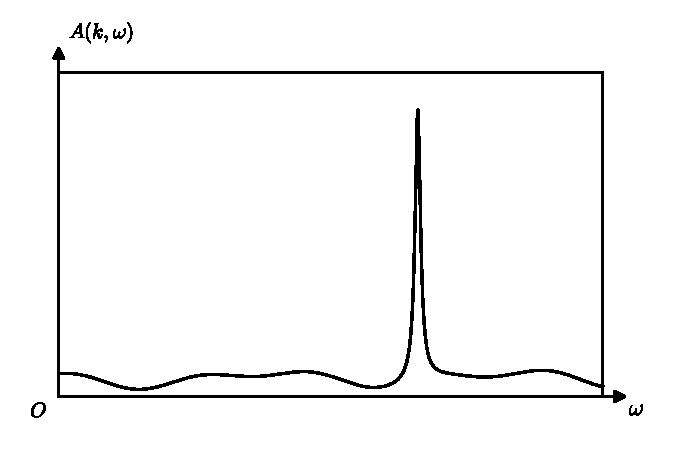
\includegraphics[width=9.5cm]{fig4-9.pdf}\\{\small 图 4.9\quad 谱函数示意图}
\end{minipage}
\end{center}

其中第二项
\begin{equation}
  g_{k}\equiv\int_{-\infty}^{\mu}A_{1}(k,\omega)\,\mathrm{d}\omega>0
\end{equation}
由于 $A_{1}$ 的正定性，其积分 $g_{k}$ 也应为正，又由于 $A_{1}$ 是 $\omega$ 的平滑函数，$g_{k}$ 也应为平滑函数，当 $k$ 越过费密面时，$g_{k}$ 应当是连续的，而式(4.11.36)右边第一项则是间断的
\begin{equation}
\begin{aligned}
  \widetilde{n}_{k}
  &=Z_{k}\int_{-\infty}^{\mu}
  \frac{\left(\varGamma_{k}/\pi\right)}
  {\left(\omega-\widetilde{E}_{k}\right)^{2}+\varGamma_{k}^{2}}\,\mathrm{d}\omega\\
  &=Z_{k}\int_{-\infty}^{\left(\mu-\widetilde{E}_{k}\right)/\varGamma_{k}}
  \frac{\mathrm{d}x}{1+x^{2}}\\
  &=Z_{k}\theta\left(\mu-\widetilde{E}_{k}\right)
  =\left\{\begin{array}{ll}
  Z_{k} & \left(\widetilde{E}_{k}<\mu\right)\\
  0 & \left(\widetilde{E}_{k}>\mu\right)
  \end{array}\right.
\end{aligned}
\end{equation}
其中利用了准粒子存在的条件 $|\widetilde{E}_{k}-\mu|\gg\varGamma_{k}$. 因此，当 $\widetilde{E}_{k}<\mu$ 时第二个等式中的积分上限可取为 $+\infty$，反之当 $\widetilde{E}_{k}>\mu$ 时取 $-\infty$，最后得到
\begin{equation}
  n_{k\sigma}=Z_{k}\theta\left(\mu-\widetilde{E}_{k}\right)+g_{k}
\end{equation}
显然，在越过费密面时准粒子的占据数有不连续的变化，其变化的大小为 $Z_{k}$，由于 $g_{k}$ 为正，而零温时 $n_{k\sigma}$ 的最大取值等于1，因此 $Z_{k}<1$. 图4.10中实线表示相互作用电子系统中占据数的动量分布示意曲线，而虚线则是熟知的零温费密分布
\begin{equation}
  n_{k\sigma}^{(0)}=\theta\left(\mu-E_{k}\right)=\theta\left(k_{\mathrm{F}}-k\right)
\end{equation}
代表自由电子的占据数分布，当越过 $k_{\mathrm{F}}$ 时，出现高度为1的台阶式间断，对应于无相互作用电子系统中存在明确的费密面.对于相互作用系统，这一明显的间断性依然存在，仅仅是间断值有所减小 $\left(Z_{k}<1\right)$，说明在 $k$ 空间仍然存在费密面.实验上，爱森伯格（Eisenberger）等人\textsuperscript{[20]}利用 X 射线的康普顿散射，在金属 Na 中已观察到占据数的明显间断，并证实了实际金属（带电）中确实存在费密面.

\begin{center}
\begin{minipage}{9.5cm}
\centering
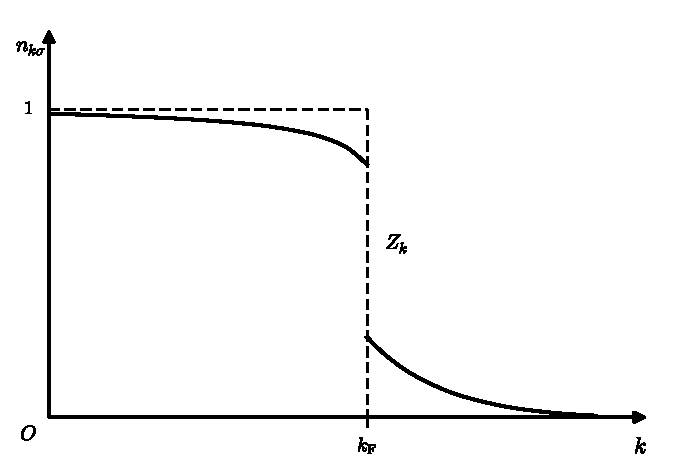
\includegraphics[width=9.5cm]{fig4-10.pdf}\\{\small 图4.10\quad 相互作用电子系中占据数的动量分布}
\end{minipage}
\end{center}

\begin{canKao}
\begin{enumerate}[label={[\arabic*]}, leftmargin=2.2em, itemsep=0pt]
\item 李正中. 相互作用费密系. 见: 蔡建华等编. 量子统计的格林函数理论. 北京: 科学出版社, 1983. 第4章
\item Nakajima S et al. The Physics of Elementary Excitation. New York: Springer-Verlag, 1980. Chap 3
\item Kubo R. J Phys Soc Japan, 1957, 12: 570
\item Fetter A L, Walecka J D. Quantum Theory of Many Particle System. New York: McGraw-Hill, 1971. Chap 4
\item Grimes C C et al. Phys Rev Lett, 1979, 42: 795
\item Halperin B I. Helv Phys Acta, 1983, 56: 75
\item Pines D. Solid State Phys, 1995, 1: 387
\item 孙鑫. 低维合作现象. 见: 郝柏林等编. 统计物理学进展. 北京: 科学出版社, 1981
\item Langer J S, Vosko S H. J Phys Chem Solids, 1960, 12: 196
\item Friedel J. Nuovo Cimento, 1958, 7 (suppl): 287
\item Gell-Mann M, Bruckner K A. Phys Rev, 1957, 106: 364
\item Hubbard J. Phys Rev, 1967, 25A: 709
\item Singwi K S et al. Phys Rev, 1970, B1: 1044
\item Wigner E. Trans Faraday Soc, 1938, 34: 678
\item Khurana A. Physics Today, 1990, 43: 17
\item Sholl C A. Proc Phys Soc (London), 1967, 92: 434
\item Nozieres P, Pines D. Phys Rev, 1958, 111: 442
\item Quinn J J, Ferrell R A. Phys Rev, 1958, 112: 812
\item Luttinger J M. Phys Rev, 1960, 119: 1153
\item Eisenberger P L et al. Phys Rev, 1972, B6: 3671
\end{enumerate}
\end{canKao}
